% ==============================================================
% Kapitola: Experimentálna analýza bezpečnostných profilov
% ==============================================================

\section{Experimentálna analýza bezpečnostných profilov}
\label{sec:experiments}

Táto kapitola nadväzuje na teoretické východiská z oblastí AEAD, správy nonce, anti-replay ochrany, derivácie kľúčov a detekcie protokolových anomálií. Kým teoretická časť formulovala bezpečnostné požiadavky a model hrozieb, táto kapitola tieto požiadavky premieňa na merateľné tvrdenia a overuje ich experimentálne pomocou profilov A1/A2\,$\times$\,R0/R1/R2. Jadrom analýzy nie je všeobecná bezpečnosť celého informačného systému, ale konkrétne vyhodnotenie toho, ako voľba AEAD algoritmu, nonce stratégie a runtime detektora ovplyvňuje odolnosť voči zvoleným triedam útokov. Každý scenár (S1--S5) priamo zodpovedá jednému teoretickému konceptu: S1 overuje anti-replay, S2 AAD binding, S3 kryptografickú izoláciu kľúčov medzi čítačkami (HKDF), S4 sekvenčnú čerstvosť a S5 forgery resistance.

Predchádzajúce kapitoly opísali návrh a implementáciu bezpečnostných mechanizmov prototypu. Cieľom tejto kapitoly je experimentálne overiť, či a ako tieto mechanizmy skutočne zvyšujú odolnosť systému voči vybraným útokovým scenárom. Experimenty sú navrhnuté tak, aby pokrývali rôzne triedy hrozieb a umožnili porovnanie šiestich konfiguračných profilov.

Výber scenárov vychádza z modelu hrozieb STRIDE\cite{STRIDE} presentovaného v teoretickej časti. Nie všetky kategórie STRIDE sú pre tento prototyp rovnako relevantné: Denial of Service je čiastočne riešený na úrovni validácie vstupov a nie je predmetom kryptografickej analýzy; Elevation of Privilege sa viaže na autorizačnú politiku, nie na nonce/AEAD mechanizmus. Tabuľka~\ref{tab:stride-scenarios} zobrazuje, ktoré kategórie STRIDE pokrývajú jednotlivé scenáre.

\begin{table}[htbp]
\renewcommand{\arraystretch}{1.3}
\centering
\caption{Mapovanie STRIDE kategórií hrozieb na experimentálne scenáre}
\label{tab:stride-scenarios}
\small
\begin{tabular}{l l l p{4.5cm}}
\toprule
\textbf{STRIDE kategória} & \textbf{Scenár} & \textbf{Mechanizmus} & \textbf{Testovaná vlastnosť} \\
\midrule
Spoofing (podvrhnutie) & S5 & AEAD Poly1305 & Odolnosť voči falzifikácii ciphertextu bez znalosti kľúča. \\
Tampering (manipulácia) & S2 & AAD binding & Detekcia zmeny poľa \texttt{door\_id} v hlavičke frame. \\
Repudiation (popieranie) & --- & Audit chain & Pokrytá unit testami, nie scenárom S1--S6. \\
Information Disclosure & --- & HMAC(card\_id) & Ochrana identifikátorov; netestovaná priamo v harness. \\
Denial of Service & --- & Validácia vstupov & Mimo rozsahu kryptografickej experimentálnej matice. \\
Elevation of Privilege & --- & RBAC + binding & Pokrytá unit testami (engine\_test). \\
Replay (nad rámec STRIDE) & S1 & ReplayWindow & Opakovanie zachyteného frame. \\
Nonce enforcement & S3a & R2 detektor & Overenie, či R2 zachytí odchýlku od deterministického nonce invariantu. \\
Key isolation (cross-reader) & S3b & HKDF + AEAD & Izolácia kľúčov medzi čítačkami --- frame z kontextu inej čítačky je odmietnutý. \\
Seq. rollback & S4 & R2 detektor & Rollback sekvenčného čísla mimo sliding window. \\
Throughput & S6 & --- & Výkonnostný overhead bezpečnostných mechanizmov. \\
\bottomrule
\end{tabular}
\end{table}

\noindent Scenáre S3, S4 a S6 nemajú priamu analógiu v STRIDE, ale pokrývajú hrozby špecifické pre protokoly s per-reader deriváciou kľúčov, rollback sekvencie a výkonnostný dopad mechanizmov. S3 vychádza z princípu kryptografickej izolácie prostredníctvom HKDF\cite{RFC5869}; S4 z literatúry o nonce misuse a odolnosti protokolov\cite{RogawayNonceMisuse2004,BellareNonceMisuse2006}.

\subsection{Matica konfiguračných profilov}
\label{sec:profile_matrix}

Experimentálny harness kombinuje dva šifrovacie algoritmy s tromi režimami generovania nonce, čo vytvára maticu šiestich profilov:

\begin{table}[htbp]
\renewcommand{\arraystretch}{1.3}
\centering
\caption{Matica konfiguračných profilov (algoritmus $\times$ režim nonce)}
\label{tab:profile_matrix}
\begin{tabular}{l c c c}
\toprule
& \textbf{R0} (random) & \textbf{R1} (deterministic) & \textbf{R2} (det. + detector) \\
\midrule
\textbf{A1} (ChaCha20-Poly1305) & A1--R0 & A1--R1 & A1--R2 \\
\textbf{A2} (XChaCha20-Poly1305) & A2--R0 & A2--R1 & A2--R2 \\
\bottomrule
\end{tabular}
\end{table}

\noindent Všetky profily zdieľajú rovnaký základ:

\begin{itemize}[leftmargin=*,itemsep=2pt]
  \item derivácia kľúčov cez HKDF s per-reader salt a verziovaním,
  \item plný AAD mód (celý plaintext header ako Additional Authenticated Data),
  \item anti-replay ochrana cez \emph{ReplayWindow} s kapacitou 256,
  \item verzovaný pepper pre HMAC identifikátorov kariet,
  \item enforced reader-door binding (väzba čítačky na dvere).
\end{itemize}

\noindent Rozdiely medzi profilmi spočívajú v troch dimenziách:

\begin{description}[leftmargin=*,itemsep=2pt]
  \item[Algoritmus (A1 vs.\ A2):] ChaCha20-Poly1305 (RFC~8439\cite{RFC8439}, 12-bajtový nonce) oproti XChaCha20-Poly1305\cite{XChaChaDraft} (24-bajtový nonce). Väčší nonce priestor u A2 znižuje pravdepodobnosť kolízie pri náhodnom generovaní.
  \item[Režim nonce (R0):] Nonce je generovaný pseudonáhodne pre každý frame. Server nonce neoveruje --- používa ho len na dešifrovanie.
  \item[Režim nonce (R1):] Nonce je generovaný deterministicky ako HMAC-SHA-256 kontextu hlavičky:
  $\text{nonce} = \text{HMAC}(K_{\text{nonce}}, \text{header\_context})$,
  kde $K_{\text{nonce}}$ je derivovaný cez HKDF s info \texttt{nonce-derivation-v1}. Server má rovnaký kľúč, ale nonce neoveruje.
  \item[Režim nonce (R2):] Rovnaký deterministický nonce ako R1, ale s aktívnym \emph{ProtocolAnomalyDetector}, ktorý:
  \begin{itemize}[itemsep=1pt]
    \item overuje, že nonce v hlavičke zodpovedá očakávanej hodnote (\texttt{nonce\_mismatch}),
    \item detekuje rollback sekvenčného čísla (\texttt{seq\_rollback}, prah $\delta = 100$),
    \item sleduje sériu neúspešných AEAD overení (\texttt{tag\_fail\_streak}, limit 5),
    \item pri detekcii anomálie čítačku \emph{zakaranténuje} --- všetky ďalšie frame z danej čítačky sú zamietnuté.
  \end{itemize}
\end{description}

\subsection{Architektúra experimentálneho harnessu}
\label{sec:harness}

Experimentálny harness je implementovaný v jazyku C++ a zdieľa rovnaký kryptografický kód aj rozhodovaciu logiku (\texttt{DecisionEngine}) ako produkčný server. Tým je zaručené, že experimenty merajú skutočné správanie systému, nie simuláciu oddelenú od implementácie --- prístup odporúčaný pre verifikáciu bezpečnostných vlastností\cite{NIST80053}. Harness nie je unit testom izolovanej kryptografickej funkcie ani úplným end-to-end testom vrátane siete; ide o \emph{security-oriented component test}: overuje, \emph{ako} je AEAD v systéme použité --- ako sa tvorí nonce, ako je hlavička viazaná cez AAD, ako systém reaguje na replay, rollback a odchýlky od protokolových invariantov.

\subsubsection{Hlavné komponenty}

\begin{description}[leftmargin=*,itemsep=2pt]
  \item[\texttt{ExperimentContext}:] Pre každú kombináciu (profil, attack\_n, run) vytvára čerstvú inštanciu obsahujúcu \texttt{KeyManager}, \texttt{SqliteAccessStore}, \texttt{DecisionEngine}, \texttt{ProtocolAnomalyDetector} a mapu \texttt{ReplayWindow}. Tým sa zaručuje, že stav z predchádzajúceho behu neovplyvní výsledok.
  \item[\texttt{FrameFactory}:] Generuje validné binárne frame identické s tým, čo by vytvoril produkčný server. Poskytuje aj statické metódy na manipuláciu frame (\texttt{tamperDoorId}, \texttt{tamperCiphertext}).
  \item[\texttt{MetricsCollector}:] Zapisuje výsledky do CSV s 15 stĺpcami: \texttt{profile}, \texttt{cipher\_mode}, \texttt{nonce\_mode}, \texttt{detector\_enabled}, \texttt{scenario}, \texttt{phase}, \texttt{attack\_n}, \texttt{frame\_idx}, \texttt{allowed}, \texttt{reason}, \texttt{quarantined}, \texttt{anomaly\_type}, \texttt{latency\_ns}, \texttt{seed}, \texttt{run\_idx}.
  \item[\texttt{IScenario}:] Rozhranie pre scenáre. Každý scenár implementuje metódy \texttt{name()}, \texttt{config()}, \texttt{setup()}, \texttt{buildTrialFrame()} a voliteľne \texttt{onBaselineFrame()}.
  \item[\texttt{runScenario()}:] Spoločná smyčka iterujúca cez 6~profilov $\times$ $N$~krokov $\times$ 5~behov.
\end{description}

\subsubsection{Fázy experimentu}

Každá iterácia prebieha v troch fázach:

\begin{enumerate}[leftmargin=*,itemsep=2pt]
  \item \textbf{Warmup} (200 frame, nezaznamenávaný): Naplní replay window a ustáli stav detektora.
  \item \textbf{Baseline} (200 frame, zaznamenaný): Validné frame. Slúži na meranie false reject rate a referenčnej latencie. Baseline sa opakuje pre každú kombináciu (profil, attack\_n, run) --- každá iterácia beží s čerstvým kontextom.
  \item \textbf{Trial / Attack} ($N$ frame, zaznamenaný): Scenár generuje útočné alebo meracie frame cez \texttt{buildTrialFrame()}.
\end{enumerate}

\subsubsection{Reprodukovateľnosť}

\begin{itemize}[leftmargin=*,itemsep=2pt]
  \item Každý beh $r$ ($r = 0\ldots4$) používa iný seed $42 + r$, čo zavádza medzibehová variabilitu pri zachovaní reprodukovateľnosti. Režim R0 používa \texttt{SeededNonceGenerator} s týmto seed-om namiesto \texttt{randombytes\_buf()}; každý beh je individuálne reprodukovateľný opakovaním s rovnakým seed-om.
  \item Čerstvý \texttt{ExperimentContext} (vrátane SQLite databázy) pre každú kombináciu (profil, step, run).
  \item CLI prepínače \texttt{--seed=N}, \texttt{--warmup=N}, \texttt{--baseline=N}, \texttt{--runs=N} umožňujú reprodukovateľné experimenty.
\end{itemize}

\subsubsection{Vzťah harnessu k produkčnému systému}

Harness je \emph{kontrolovaný experimentálny mini-systém}, nie plná replika produkčného servera. Zdieľa s produkčným kódom kryptografickú vrstvu (\texttt{crypto\_lib}), deriváciu kľúčov (\texttt{key\_manager}), rozhodovaciu logiku (\texttt{DecisionEngine}), anti-replay mechanizmus (\texttt{ReplayWindow}) a anomálny detektor (\texttt{ProtocolAnomalyDetector}). Zámerne sú vynechané vrstvy, ktoré nie sú predmetom merania:

\begin{itemize}[leftmargin=*,itemsep=2pt]
  \item \textbf{HTTP transport a HMAC autentifikácia požiadavky} --- harness volá \texttt{DecisionEngine::process()} priamo, bez sieťového overhead-u. Tým sa izoluje latencia kryptografických a rozhodovacích operácií od variability sieťového zásobníka.
  \item \textbf{Kontrola čerstvosti (\texttt{maxSkewMs = 0})} --- overenie časovej pečiatky je v harness vypnuté, aby sa predišlo kontaminácii výsledkov efektmi časovej synchronizácie. Experimenty sa zameriavajú na nonce, replay a detektor, nie na hodiny.
  \item \textbf{Perzistentný auditný log} --- harness používa in-memory audit sink namiesto HMAC hash chain s~SQLite perzistenciou. Auditná integrita je testovaná samostatne v~unit testoch; v~experimentoch by perzistentný zápis pridával I/O latenciu nesúvisiacu s meranými mechanizmami.
\end{itemize}

\noindent Šesť konfiguračných profilov (A1-R0 až A2-R2) je definovaných programaticky vo funkcii \texttt{allProfiles()}, nie načítaných zo súboru YAML. Hodnoty parametrov (algoritmus, režim nonce, stav detektora) sú ekvivalentné produkčným YAML konfiguráciám, ale priama definícia v~kóde eliminuje závislosť na externom súbore a zaisťuje, že profily sa nemôžu meniť medzi behmi.

\subsection{Popis útokových scenárov}
\label{sec:scenarios}

\subsubsection{S1: Replay útok}

Scenár zachytí validný frame v polovici baseline fázy a opakovane ho posiela v trial fáze. Modeluje útočníka, ktorý zachytil sieťovú komunikáciu a reprodukuje ju bez modifikácie --- štandardný replay útok podľa klasifikácie NIST\cite{NIST80098}.

\textit{Očakávané správanie:} Replay window odchytí duplikát sekvenčného čísla. R2 navyše zakaranténuje čítačku s anomáliou \texttt{seq\_reuse}.

\subsubsection{S2: Manipulácia poľa v hlavičke (AAD tampering)}

Scenár vytvorí validný frame a následne zmení \texttt{door\_id} v binárnej serializácii hlavičky bez opätovného šifrovania payloadu. Overuje AAD binding: cieľom je zachytiť nekonzistentnosť medzi hlavičkou a payloadom na úrovni kryptografickej väzby --- nie na úrovni sieťovej vrstvy alebo aplikačného smerovania.

\textit{Konfigurácia:} V harness sa podvrhnutý \texttt{door\_id} (pôvodný $+ 999$) explicitne registruje ako povolené dvere pre danú čítačku (\texttt{allowDoorForReader}). Tým sa izoluje kryptografická detekcia manipulácie od autorizačnej politiky --- bez tohto kroku by frame bol zamietnutý už na úrovni reader-door bindingu (\texttt{unknown\_reader}), čo by zakrylo správanie AEAD/AAD vrstvy.

\textit{Očakávané správanie:} Keďže \texttt{door\_id} je súčasťou AAD, zmena spôsobí zlyhanie AEAD overenia. R0/R1 vracajú \texttt{decrypt\_failed}. R2 detekuje problém skôr --- zmena \texttt{door\_id} mení kontext pre deterministický nonce, takže overenie nonce zlyhá (\texttt{nonce\_mismatch}) ešte pred pokusom o dešifrovanie.

\subsubsection{S3a: Overenie nonce enforcement politiky}

Scenár injektuje chybu do generovania nonce: \texttt{FixedNonceGenerator(0xAA)} produkuje rovnaký nonce pre každý frame bez ohľadu na kontext a sekvenciu. Cieľom je overiť, či a ako jednotlivé nonce režimy reagujú na porušenie deterministického nonce invariantu.

\textit{Očakávané správanie:} R0/R1 nemajú verifikáciu nonce --- engine použije nonce z hlavičky frame na dešifrovanie bez ďalšej kontroly. AEAD dešifrovanie uspeje (kľúč je správny, nonce je len vstupný parameter). R2 rekonštruuje očakávaný nonce z rovnakého kľúča a kontextu a porovná ho s hodnotou v hlavičke; pri nesúlade vyvolá \texttt{nonce\_mismatch} s okamžitou karanténou.

\textit{Prečo je tento test dôležitý:} S3a je jediný scenár, ktorý priamo testuje \textbf{nonce enforcement} --- odlišuje R0/R1 od R2 práve v kontexte nonce politiky (S4 odlišuje R0/R1 od R2 cez seq rollback detekciu, nie nonce). V aktuálnom jednoserverovom nasadení generátor aj verifikátor nonce zdieľajú ten istý \texttt{KeyManager} --- za normálnych okolností k odchýlke nedôjde. Avšak ak systém v budúcnosti prejde na distribuovanú architektúru (viacero serverov, oddelené generovanie a verifikácia frame, multi-process nasadenie), vynucovaná nonce politika sa stáva kritickou bezpečnostnou poistkou. R2 zabezpečuje, že štrukturálne zmeny v nasadení nenaruší garanciu unikátnosti nonce bez povšimnutia\cite{RogawayNonceMisuse2004}.

\subsubsection{S3b: Izolácia kľúčov medzi čítačkami (HKDF key isolation)}

Komponentový validačný scenár overuje, že frame vytvorený v kľúčovom kontexte jednej čítačky nemožno úspešne overiť v kontexte inej čítačky. Nejde o simuláciu aktuálneho produkčného HTTP toku zariadenia (čítačka v produkcii nekonštruuje AEAD frame), ale o overenie izolačných vlastností HKDF per-reader derivácie v AEAD vrstve.

HKDF\cite{RFC5869} derivuje unikátny kľúč pre každú čítačku:
\begin{equation}
K_{\text{aead}}^{(r)} = \text{HKDF}(\text{master}, \; \text{salt}=\text{reader\_id} \| \text{key\_version}, \; \text{info}=\text{``access-aead-v1''})
\end{equation}

\textit{Postup:} Harness zašifruje frame kľúčom čítačky~2 ($K_{\text{aead}}^{(2)}$), ale hlavičku frame podvrhne tak, aby obsahovala \texttt{reader\_id}=1. Engine parsuje hlavičku, derivuje kľúč pre čítačku~1 ($K_{\text{aead}}^{(1)}$) a pokúsi sa o AEAD dešifrovanie. Zlyhanie je dvojnásobné: kľúč aj AAD sú nekonzistentné so šifrovaným obsahom.

\textit{Očakávané správanie:} Všetky profily odmietajú 100\% útočných frame (\texttt{decrypt\_failed}). R2 navyše detekuje nonce anomáliu okamžite (nonce bol derivovaný z kontextu čítačky~2) --- \texttt{nonce\_mismatch} vedie ku karanténe od prvého frame. Kľúčový záver: HKDF per-reader derivácia poskytuje kryptografickú izoláciu (compartmentalization) --- kompromitácia jednej čítačky neohrozí ostatné.

\subsubsection{S4: Rollback sekvenčného čísla}

Scenár posiela frame so sekvenčnými číslami z ``rollback zóny'' --- hodnoty, ktoré sú nižšie ako maximálne videné číslo, ale nie sú príliš staré pre replay window a neboli nikdy odoslané.

Rollback zóna je definovaná:
\begin{equation}
\text{rollback zone} = [\text{maxSeen} - W + 1, \; \text{maxSeen} - \delta)
\end{equation}
kde $W = 256$ je veľkosť replay window a $\delta = 100$ je rollback threshold.

\textit{Očakávané správanie:} Replay window tieto sekvencie neodmietne, pretože nie sú ``too old'' ($> \text{maxSeen} - W$) ani v množine videných. R0/R1 teda čiastočne prepustia útok. R2 detekuje rollback cez podmienku $\text{seq} + \delta < \text{maxSeenSeq}$ a okamžite zakaranténuje čítačku.

\textit{Matematika úspešnosti pre R0/R1:} Z 155 slotov v rollback zóne sa 99 prekrýva s baseline sekvenciami v \texttt{\_seen} sade (60000--60098). Reálne prejde len 56 unikátnych sekvencií (59944--59999). Pri $N=500$: $56/500 = 11.2\%$.

\subsubsection{S5: Tag probe (forgery resistance)}

Scenár vytvorí validný frame a následne poškodí ciphertext náhodnými bajtami. Overuje, či AEAD tag verifikácia zachytí poškodenú šifrovanú časť frame --- formálne ide o test odolnosti použitia AEAD voči forgery pokusom\cite{RFC5116}. Nejde o modelovanie externého útočníka, ktorý posiela ciphertext po sieti; frame je interná štruktúra servera. Scenár testuje správanie overenia tagu pri chybnom alebo zámernom poškodení v rámci spracovacej cesty.

\textit{Očakávané správanie:} AEAD overenie zlyhá pre všetky profily (\texttt{decrypt\_failed}). R2 navyše sleduje sériu zlyhaní a po dosiahnutí limitu 5 zakaranténuje čítačku s anomáliou \texttt{tag\_fail\_streak}.

\subsubsection{S6: Throughput benchmark}

Čisto výkonnostný scenár. Posiela len validné frame (detektor sa neaktivuje). Meria latenciu spracovania a priepustnosť.

\begin{itemize}[leftmargin=*,itemsep=2pt]
  \item Warmup: 1000 frame, baseline: 0, trial: 1000/5000/10000/50000 frame.
  \item 5 behov s odlišnými seed-mi (42--46) na posúdenie variability a robustnosti výsledkov naprieč behmi.
  \item Fáza trial označená ako ``measure'' (nie ``attack'').
\end{itemize}

\subsection{Metodika zberu a spracovania dát}
\label{sec:methodology}

\subsubsection{Zber dát}

Každý scenár produkuje CSV súbor s jedným riadkom na frame. Celkový objem dát pri 5 behoch: ${\sim}2{,}835{,}000$ riadkov. Pre každý frame sa zaznamenáva:

\begin{itemize}[leftmargin=*,itemsep=2pt]
  \item konfiguračný profil a jeho parametre,
  \item fáza (baseline/attack/measure), počet útočných frame a index behu,
  \item rozhodnutie (\texttt{allowed}), dôvod (\texttt{reason}), stav karantény,
  \item typ anomálie (ak bola detekovaná detektorom),
  \item latencia spracovania v nanosekundách.
\end{itemize}

\subsubsection{Odvodzované metriky}

Z primárnych dát sa počítajú nasledujúce metriky:

\begin{description}[leftmargin=*,itemsep=2pt]
  \item[Attack success rate:] Podiel útočných frame, ktoré boli povolené ($\texttt{allowed} = \text{true}$), agregovaný cez behy (priemer $\pm$ smerodajná odchýlka).
  \item[False reject rate:] Podiel baseline frame, ktoré boli zamietnuté (meria falošné odmietnutia validných požiadaviek).
  \item[Time to quarantine:] Index prvého frame, kde bol čítač zakaranténovaný (len R2 profily).
  \item[Throughput:] $\text{FPS} = \frac{\text{počet frame}}{\sum \text{latencia\_ns} / 10^9}$, počítaný per (profil, $N$, beh).
  \item[Latencia:] Percentily p50, p95, p99 v $\mu$s.
\end{description}

\subsubsection{Štatistická robustnosť}

Každý beh $r$ ($r = 0\ldots4$) používa seed $42 + r$, takže nonce hodnoty sa líšia medzi behmi. Pre \textbf{bezpečnostné metriky} (S1--S5) 5 behov slúži ako kontrola reprodukovateľnosti: keďže ochranné mechanizmy (AEAD overenie, replay window, detektor) sú invariantné voči konkrétnym hodnotám nonce, výsledok je binárny a zhodný naprieč všetkými behmi. Pásma v grafoch majú nulovú šírku --- nie ako výsledok štatistickej inferencie, ale ako vizuálne potvrdenie konzistentnosti. Pre \textbf{latenciu a priepustnosť} (S6) sú behy skutočným zdrojom variability (OS a HW šum) a štandardná odchýlka má bežný štatistický výklad; dosahuje 1--4\,\% priemeru.

\subsection{Výsledky: Úspešnosť útokov}
\label{sec:results_attacks}

\subsubsection{Celkový prehľad}

Obrázok~\ref{fig:heatmap} zobrazuje úspešnosť útokov pre všetky kombinácie scenár $\times$ profil pri maximálnom počte útočných frame ($N=500$, resp.\ $N=50{,}000$ pre S6).

\begin{figure}[htbp]
\centering
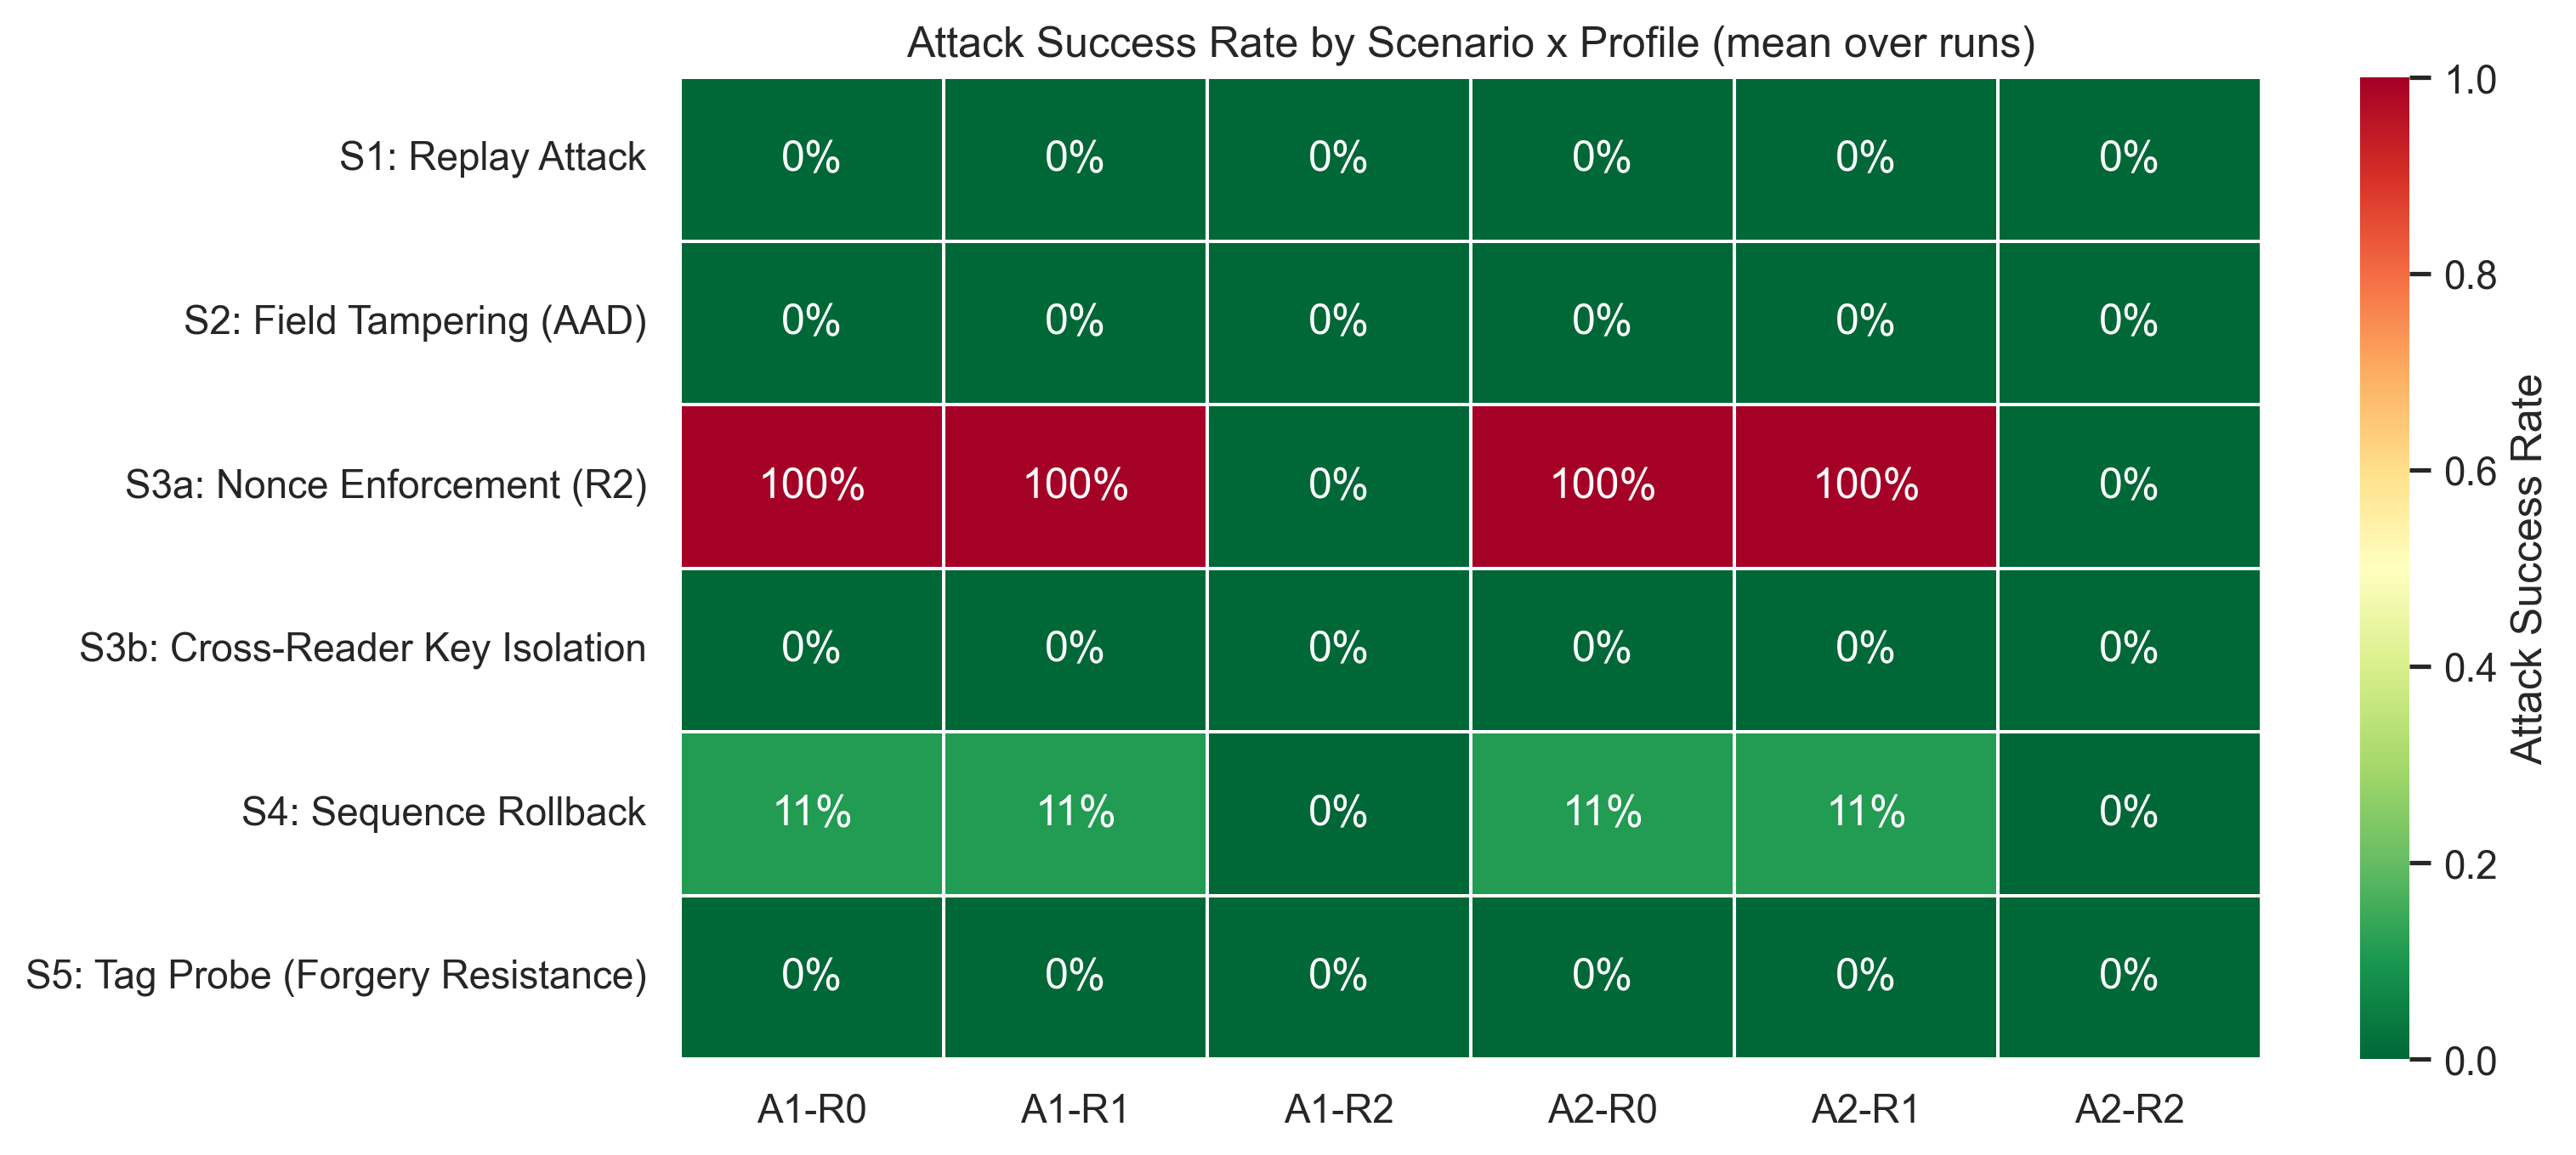
\includegraphics[width=\linewidth]{plots/attack_success_heatmap.png}
\caption{Úspešnosť útokov podľa scenára a profilu (priemer cez 5 behov). Zelené bunky: útok zablokovaný (0\%). Červené bunky: útok úspešný.}
\label{fig:heatmap}
\end{figure}

\begin{table}[htbp]
\centering
\caption{Attack success rate and detector response by scenario and profile}
\label{tab:scenario-summary}
\small
\begin{tabular}{l l r c l l}
\toprule
Scenario & Profile & Success \% & Quarantine & Reason & Anomaly \\
\midrule
  S1: Replay Attack & A1--R0 & 0\% & No & \texttt{replay} & \texttt{--} \\
   & A1--R1 & 0\% & No & \texttt{replay} & \texttt{--} \\
   & A1--R2 & 0\% & Yes & \texttt{quarantined} & \texttt{seq\_reuse} \\
   & A2--R0 & 0\% & No & \texttt{replay} & \texttt{--} \\
   & A2--R1 & 0\% & No & \texttt{replay} & \texttt{--} \\
   & A2--R2 & 0\% & Yes & \texttt{quarantined} & \texttt{seq\_reuse} \\
\midrule
  S2: Field Tampering (AAD) & A1--R0 & 0\% & No & \texttt{decrypt\_failed} & \texttt{--} \\
   & A1--R1 & 0\% & No & \texttt{decrypt\_failed} & \texttt{--} \\
   & A1--R2 & 0\% & Yes & \texttt{quarantined} & \texttt{nonce\_mismatch} \\
   & A2--R0 & 0\% & No & \texttt{decrypt\_failed} & \texttt{--} \\
   & A2--R1 & 0\% & No & \texttt{decrypt\_failed} & \texttt{--} \\
   & A2--R2 & 0\% & Yes & \texttt{quarantined} & \texttt{nonce\_mismatch} \\
\midrule
  S3a: Nonce Enforcement (R2) & A1--R0 & 100\% & No & \texttt{ok} & \texttt{--} \\
   & A1--R1 & 100\% & No & \texttt{ok} & \texttt{--} \\
   & A1--R2 & 0\% & Yes & \texttt{quarantined} & \texttt{nonce\_mismatch} \\
   & A2--R0 & 100\% & No & \texttt{ok} & \texttt{--} \\
   & A2--R1 & 100\% & No & \texttt{ok} & \texttt{--} \\
   & A2--R2 & 0\% & Yes & \texttt{quarantined} & \texttt{nonce\_mismatch} \\
\midrule
  S3b: Cross-Reader Key Isolation & A1--R0 & 0\% & No & \texttt{decrypt\_failed} & \texttt{--} \\
   & A1--R1 & 0\% & No & \texttt{decrypt\_failed} & \texttt{--} \\
   & A1--R2 & 0\% & Yes & \texttt{quarantined} & \texttt{nonce\_mismatch} \\
   & A2--R0 & 0\% & No & \texttt{decrypt\_failed} & \texttt{--} \\
   & A2--R1 & 0\% & No & \texttt{decrypt\_failed} & \texttt{--} \\
   & A2--R2 & 0\% & Yes & \texttt{quarantined} & \texttt{nonce\_mismatch} \\
\midrule
  S4: Sequence Rollback & A1--R0 & 11\% & No & \texttt{replay} & \texttt{--} \\
   & A1--R1 & 11\% & No & \texttt{replay} & \texttt{--} \\
   & A1--R2 & 0\% & Yes & \texttt{quarantined} & \texttt{seq\_rollback} \\
   & A2--R0 & 11\% & No & \texttt{replay} & \texttt{--} \\
   & A2--R1 & 11\% & No & \texttt{replay} & \texttt{--} \\
   & A2--R2 & 0\% & Yes & \texttt{quarantined} & \texttt{seq\_rollback} \\
\midrule
  S5: Tag Probe (Forgery Resistance) & A1--R0 & 0\% & No & \texttt{decrypt\_failed} & \texttt{--} \\
   & A1--R1 & 0\% & No & \texttt{decrypt\_failed} & \texttt{--} \\
   & A1--R2 & 0\% & Yes & \texttt{quarantined} & \texttt{--} \\
   & A2--R0 & 0\% & No & \texttt{decrypt\_failed} & \texttt{--} \\
   & A2--R1 & 0\% & No & \texttt{decrypt\_failed} & \texttt{--} \\
   & A2--R2 & 0\% & Yes & \texttt{quarantined} & \texttt{--} \\
\bottomrule
\end{tabular}
\end{table}

\noindent Z tabuľky~\ref{tab:scenario-summary} a obrázka~\ref{fig:heatmap} vyplýva jasné delenie:

\begin{itemize}[leftmargin=*,itemsep=2pt]
  \item \textbf{S1, S2, S5} --- pri žiadnom profile nedošlo k prijatiu škodlivého frame (0\% úspešnosť). Ochranu zabezpečuje replay window (S1), AAD binding (S2) a AEAD tag verifikácia (S5).
  \item \textbf{S3a} --- nonce enforcement: R0/R1 prepustia frame s chybným nonce (100\%); R2 odchýlku zachytí a zakaranténuje (0\%).
  \item \textbf{S3b} --- cross-reader key isolation: žiadny profil neprijal frame z kontextu inej čítačky (0\%); R2 karanténuje od prvého frame.
  \item \textbf{S4} --- R0/R1 čiastočne zraniteľné (11\%), R2 blokuje (0\%).
\end{itemize}

\subsubsection{Závislosť od počtu útočných frame}

Obrázok~\ref{fig:by_n} zobrazuje ako sa úspešnosť útoku mení s rastúcim $N$. Pásma zobrazujú 95\% interval spoľahlivosti cez 5 behov; nulová šírka pásiem potvrdzuje konzistentnosť výsledkov naprieč všetkými behmi.

\begin{figure}[htbp]
\centering
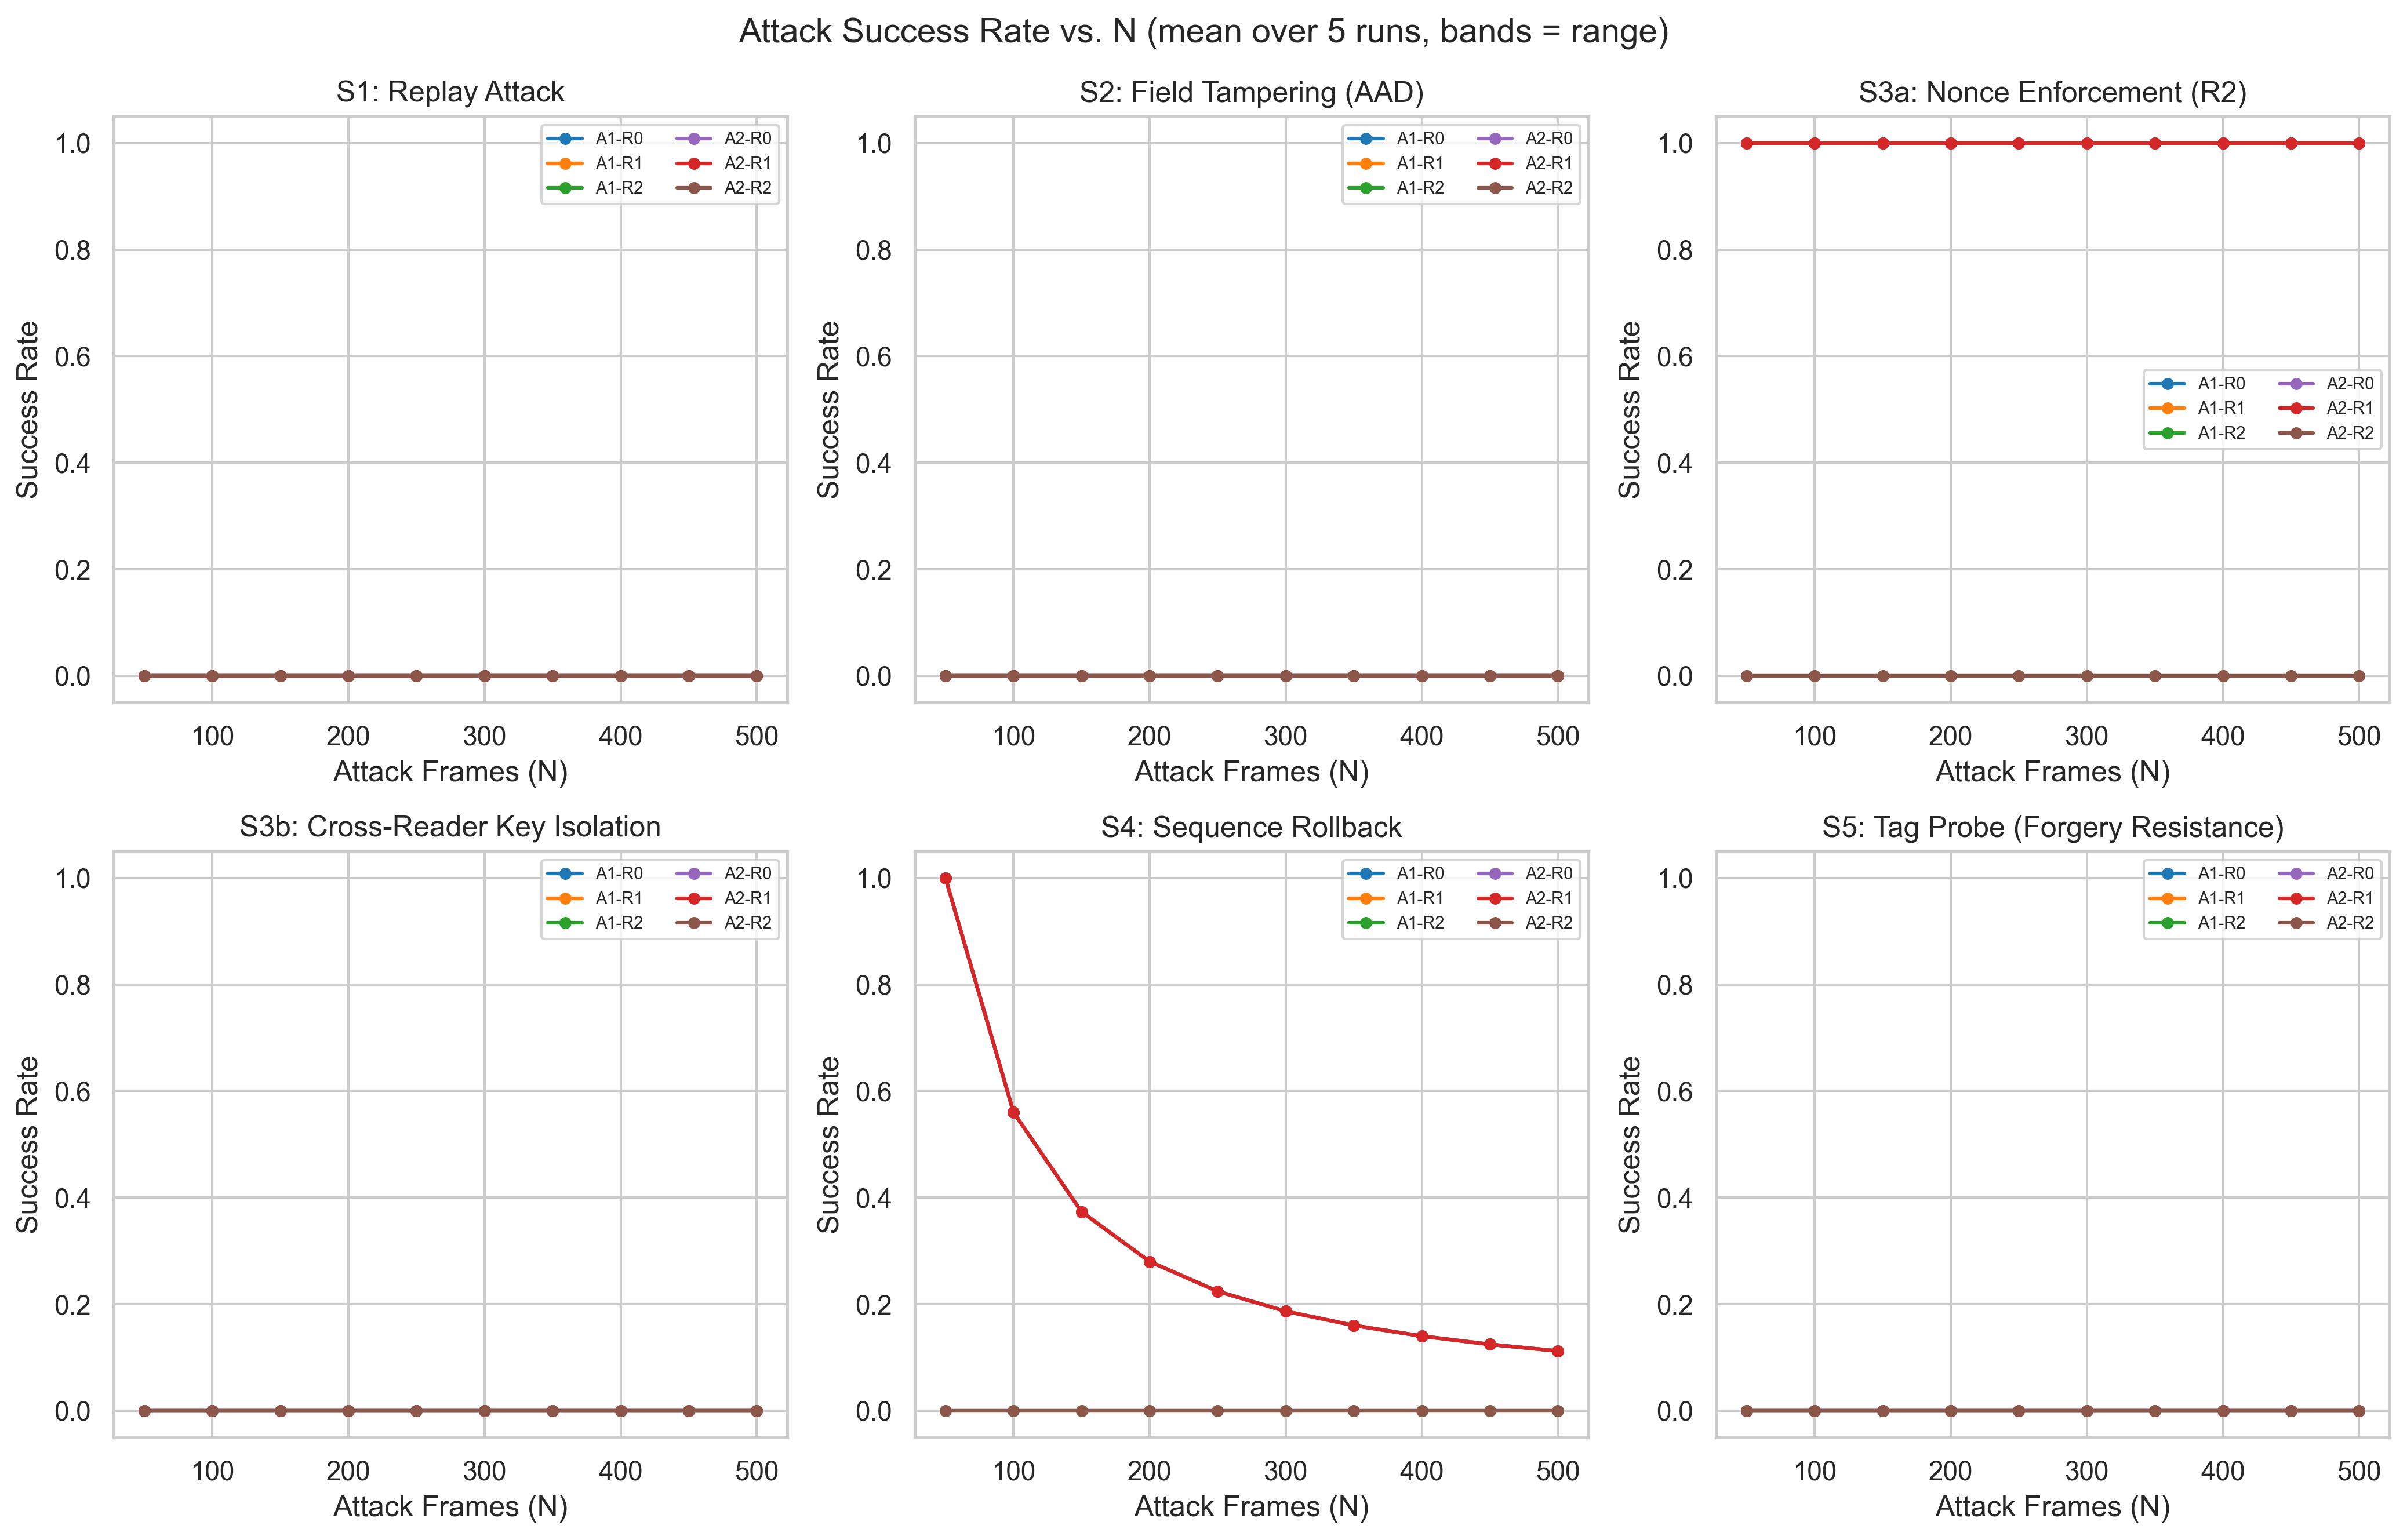
\includegraphics[width=\linewidth]{plots/attack_success_by_n.png}
\caption{Závislosť úspešnosti útoku od počtu útočných frame $N$. Pásma: 95\% CI cez 5 behov (nulová šírka = konzistentný deterministický výsledok).}
\label{fig:by_n}
\end{figure}

\noindent Najzaujímavejší je graf S4 (Sequence Rollback): úspešnosť R0/R1 klesá z ${\sim}100\%$ pri $N=50$ na ${\sim}11\%$ pri $N=500$, pretože rollback zóna obsahuje len 56 unikátnych sekvencií --- po ich vyčerpaní replay window odchytáva opakované hodnoty. R2 profily vykazujú konštantnú nulovú úspešnosť pre všetky $N$.

\subsubsection{Rýchlosť karantény}

\begin{figure}[htbp]
\centering
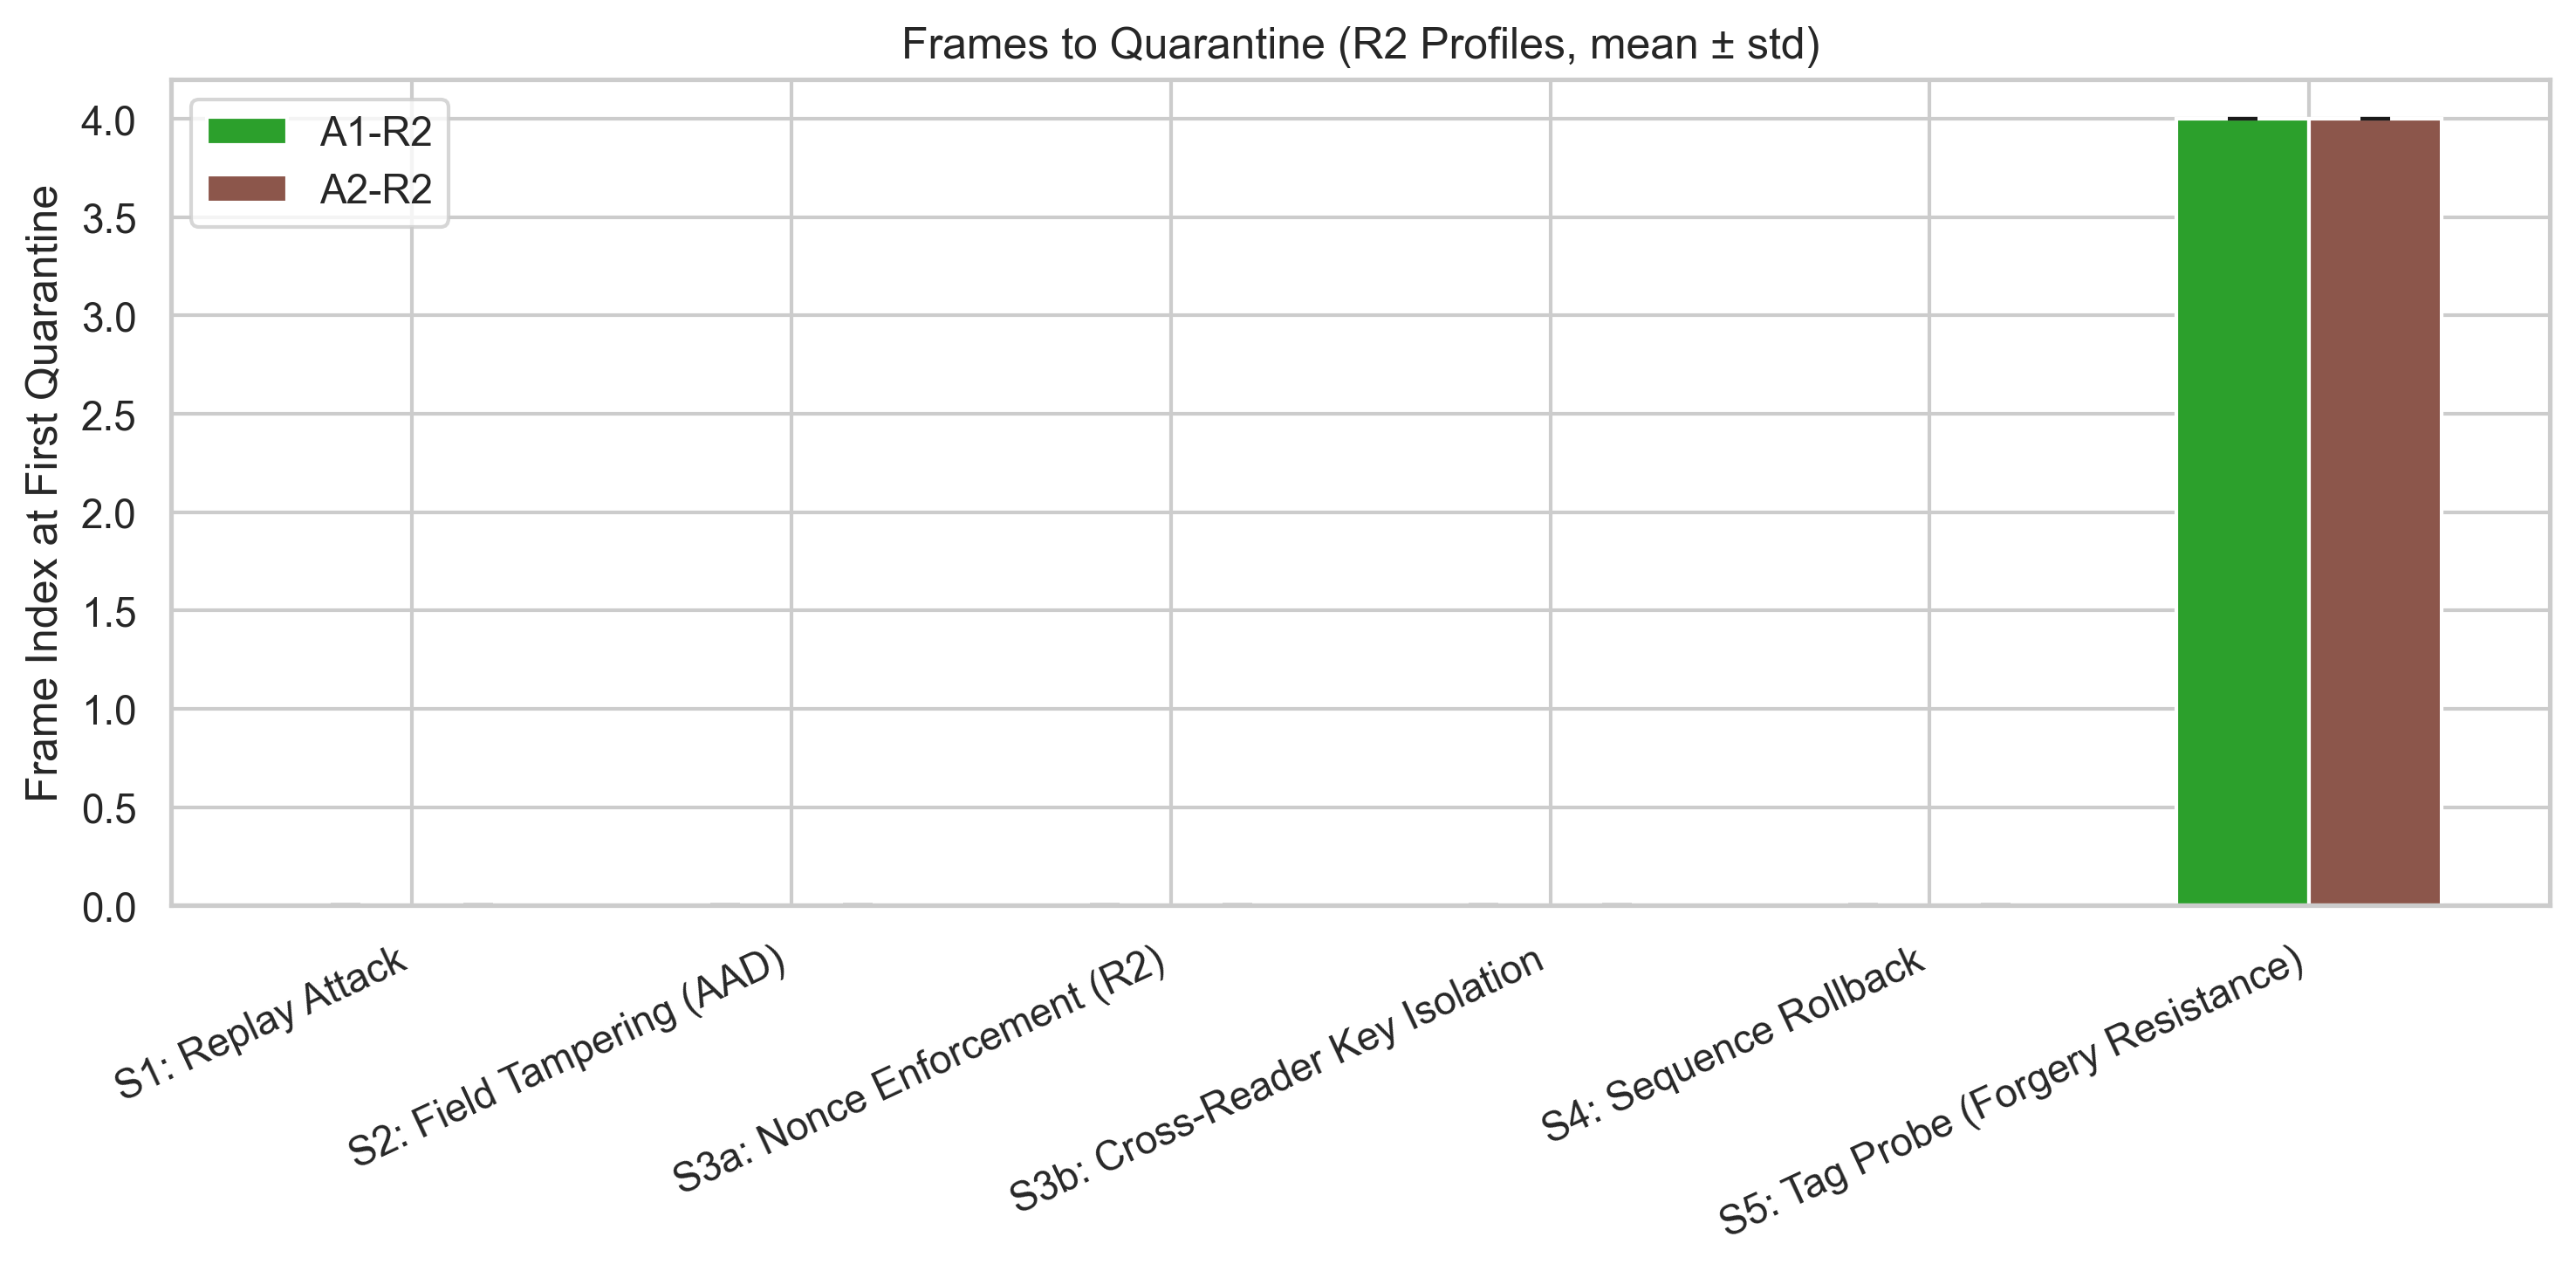
\includegraphics[width=\linewidth]{plots/quarantine_speed.png}
\caption{Počet frame od začiatku útoku do prvej karantény (len R2 profily, priemer $\pm$ std).}
\label{fig:quarantine}
\end{figure}

Obrázok~\ref{fig:quarantine} ukazuje, že pre scenáre S1--S4 nastáva karanténa \emph{na prvom útočnom frame} (frame\_idx = 0). Pre S5 (tag probe) nastáva na frame\_idx = 4, čo zodpovedá nakonfigurovanému limitu \texttt{tag\_fail\_streak\_limit} = 5 (prvé 4 zlyhania sú tolerované; 5.\ zlyhanie aktivuje karanténu). Hodnoty A1--R2 a A2--R2 sú identické, čo potvrdzuje, že rýchlosť detekcie závisí od konfigurácie detektora, nie od zvoleného šifrovacieho algoritmu.

\subsection{Výsledky: Baseline korektnosť}
\label{sec:results_baseline}

\begin{table}[htbp]
\centering
\caption{False reject rate during baseline (valid frames)}
\label{tab:baseline}
\begin{tabular}{l r r r r r r}
\toprule
Scenario & A1--R0 & A1--R1 & A1--R2 & A2--R0 & A2--R1 & A2--R2 \\
\midrule
  S1: Replay Attack & 0.00\% & 0.00\% & 0.00\% & 0.00\% & 0.00\% & 0.00\% \\
  S2: Field Tampering (AAD) & 0.00\% & 0.00\% & 0.00\% & 0.00\% & 0.00\% & 0.00\% \\
  S3a: Nonce Enforcement (R2) & 0.00\% & 0.00\% & 0.00\% & 0.00\% & 0.00\% & 0.00\% \\
  S3b: Cross-Reader Key Isolation & 0.00\% & 0.00\% & 0.00\% & 0.00\% & 0.00\% & 0.00\% \\
  S4: Sequence Rollback & 0.00\% & 0.00\% & 0.00\% & 0.00\% & 0.00\% & 0.00\% \\
  S5: Tag Probe (Forgery Resistance) & 0.00\% & 0.00\% & 0.00\% & 0.00\% & 0.00\% & 0.00\% \\
\bottomrule
\end{tabular}
\end{table}

\noindent Tabuľka~\ref{tab:baseline} potvrdzuje \textbf{nulovú false reject rate} naprieč všetkými scenármi a profilmi. Žiadny validný frame nebol zamietnutý. Toto je nevyhnutná podmienka pre vierohodnosť bezpečnostných výsledkov --- ak by baseline vykazoval falošné odmietnutia, nebolo by možné jednoznačne interpretovať úspešnosť útokov.

\subsection{Výsledky: Latencia a priepustnosť}
\label{sec:results_throughput}

\subsubsection{Throughput benchmark (S6)}

\begin{figure}[htbp]
\centering
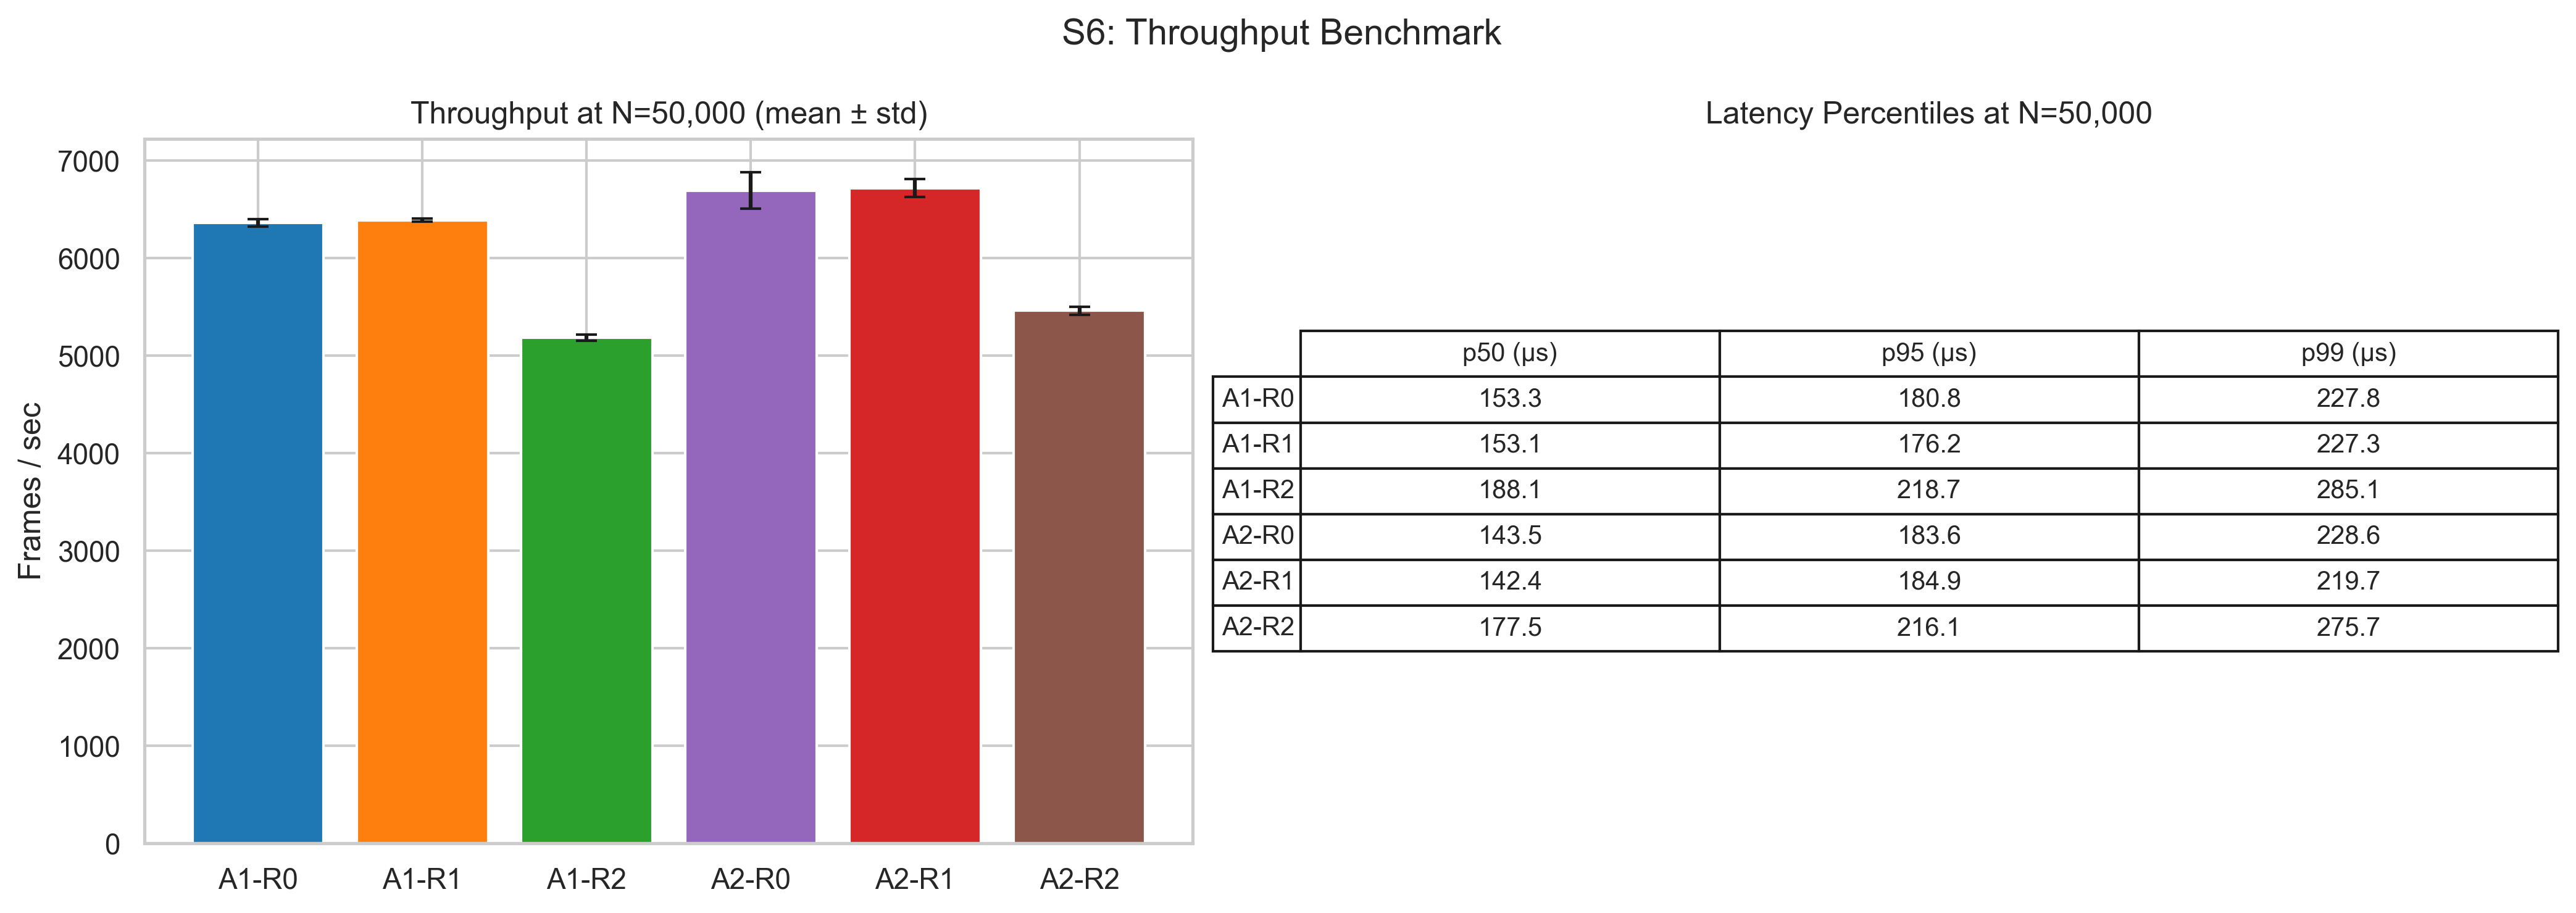
\includegraphics[width=\linewidth]{plots/throughput.png}
\caption{Priepustnosť pri $N=50{,}000$ frame (priemer $\pm$ std cez 5 behov) a percentily latencie.}
\label{fig:throughput}
\end{figure}

\begin{table}[htbp]
\centering
\caption{Throughput and latency at N=50,000 frames}
\label{tab:throughput}
\begin{tabular}{l r r r r r}
\toprule
Profile & FPS (mean) & FPS (std) & p50 ($\mu$s) & p95 ($\mu$s) & p99 ($\mu$s) \\
\midrule
  A1--R0 & 14,284 & 274 & 59.3 & 109.6 & 117.2 \\
  A1--R1 & 16,014 & 680 & 58.4 & 92.3 & 111.5 \\
  A1--R2 & 15,154 & 210 & 62.7 & 88.3 & 113.8 \\
  A2--R0 & 16,529 & 72 & 56.6 & 87.1 & 105.4 \\
  A2--R1 & 17,015 & 67 & 56.7 & 72.2 & 95.9 \\
  A2--R2 & 15,306 & 164 & 62.5 & 86.1 & 106.9 \\
\bottomrule
\end{tabular}
\end{table}

\noindent Obrázok~\ref{fig:throughput} zobrazuje distribúciu priepustnosti pre každý profil. Všetky profily dosahujú priepustnosť nad 5{,}000 frame/s, čo je rádovo viac ako reálna záťaž fyzického prístupového systému ($<$10 udalostí/s). Mediánová latencia je 142--188\,$\mu$s.

\textbf{Porovnanie algoritmov:} A2 (XChaCha20) dosahuje mierne vyššiu priepustnosť ako A1 (ChaCha20), čo je prekvapivý výsledok. Príčinou je pravdepodobne optimalizácia libsodium pre XChaCha20 cestu.

\textbf{Overhead detektora:} Porovnanie R1 a R2 umožňuje izolovať overhead \texttt{ProtocolAnomalyDetector}. Rozdiel je ${\sim}19\%$ (A2--R1: 6{,}720~fps vs.\ A2--R2: 5{,}462~fps). Tento overhead pochádza z:
\begin{itemize}[leftmargin=*,itemsep=1pt]
  \item výpočtu očakávaného nonce (HKDF derivácia + HMAC),
  \item porovnania nonce v konštantnom čase (\texttt{sodium\_memcmp}),
  \item aktualizácie stavu detektora (rollback check, tag streak).
\end{itemize}

\subsubsection{Overhead detektora na baseline frame}

\begin{figure}[htbp]
\centering
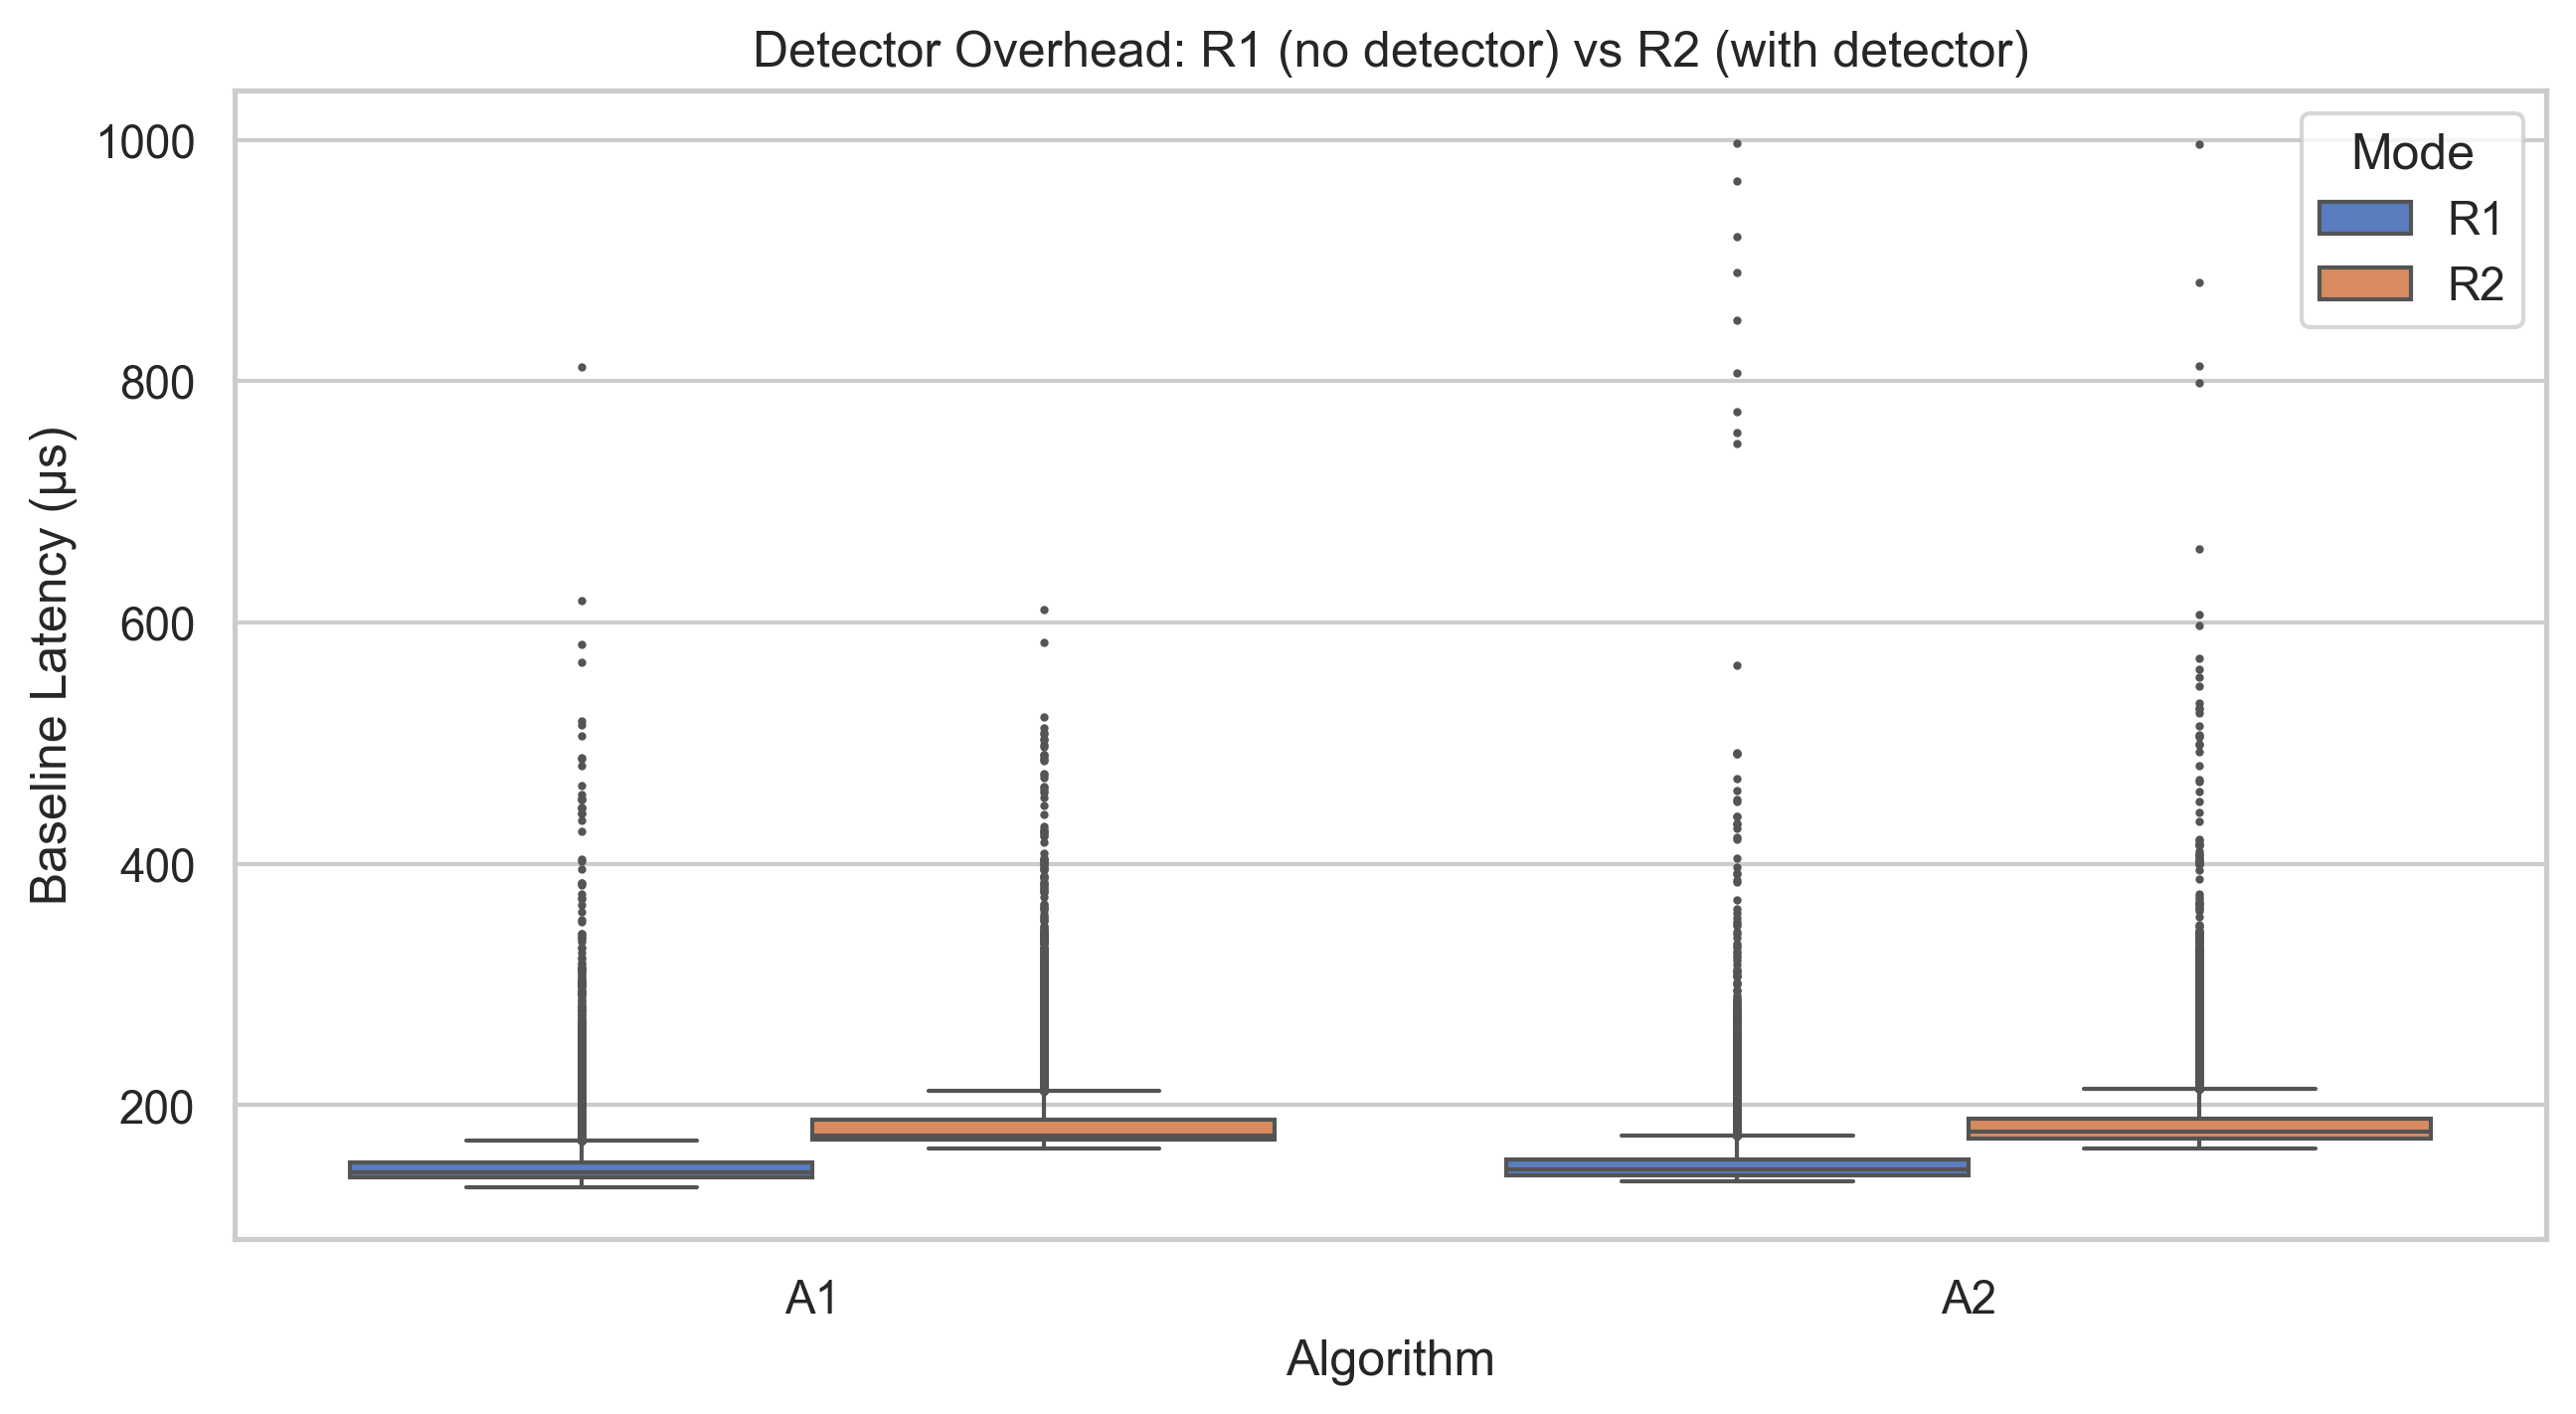
\includegraphics[width=\linewidth]{plots/detector_overhead.png}
\caption{Porovnanie latencie R1 (bez detektora) a R2 (s detektorom) na validných baseline frame.}
\label{fig:overhead}
\end{figure}

\noindent Obrázok~\ref{fig:overhead} izoluje overhead detektora porovnaním R1 a R2 na baseline frame z S1--S5. Medián latencie R2 je o ${\sim}35\,\mu$s vyšší, čo zodpovedá dodatočnej HKDF derivácii nonce kľúča, HMAC výpočtu pre overenie nonce a aktualizácii stavu detektora.

\subsubsection{Distribúcia latencie podľa scenárov}

\begin{figure}[htbp]
\centering
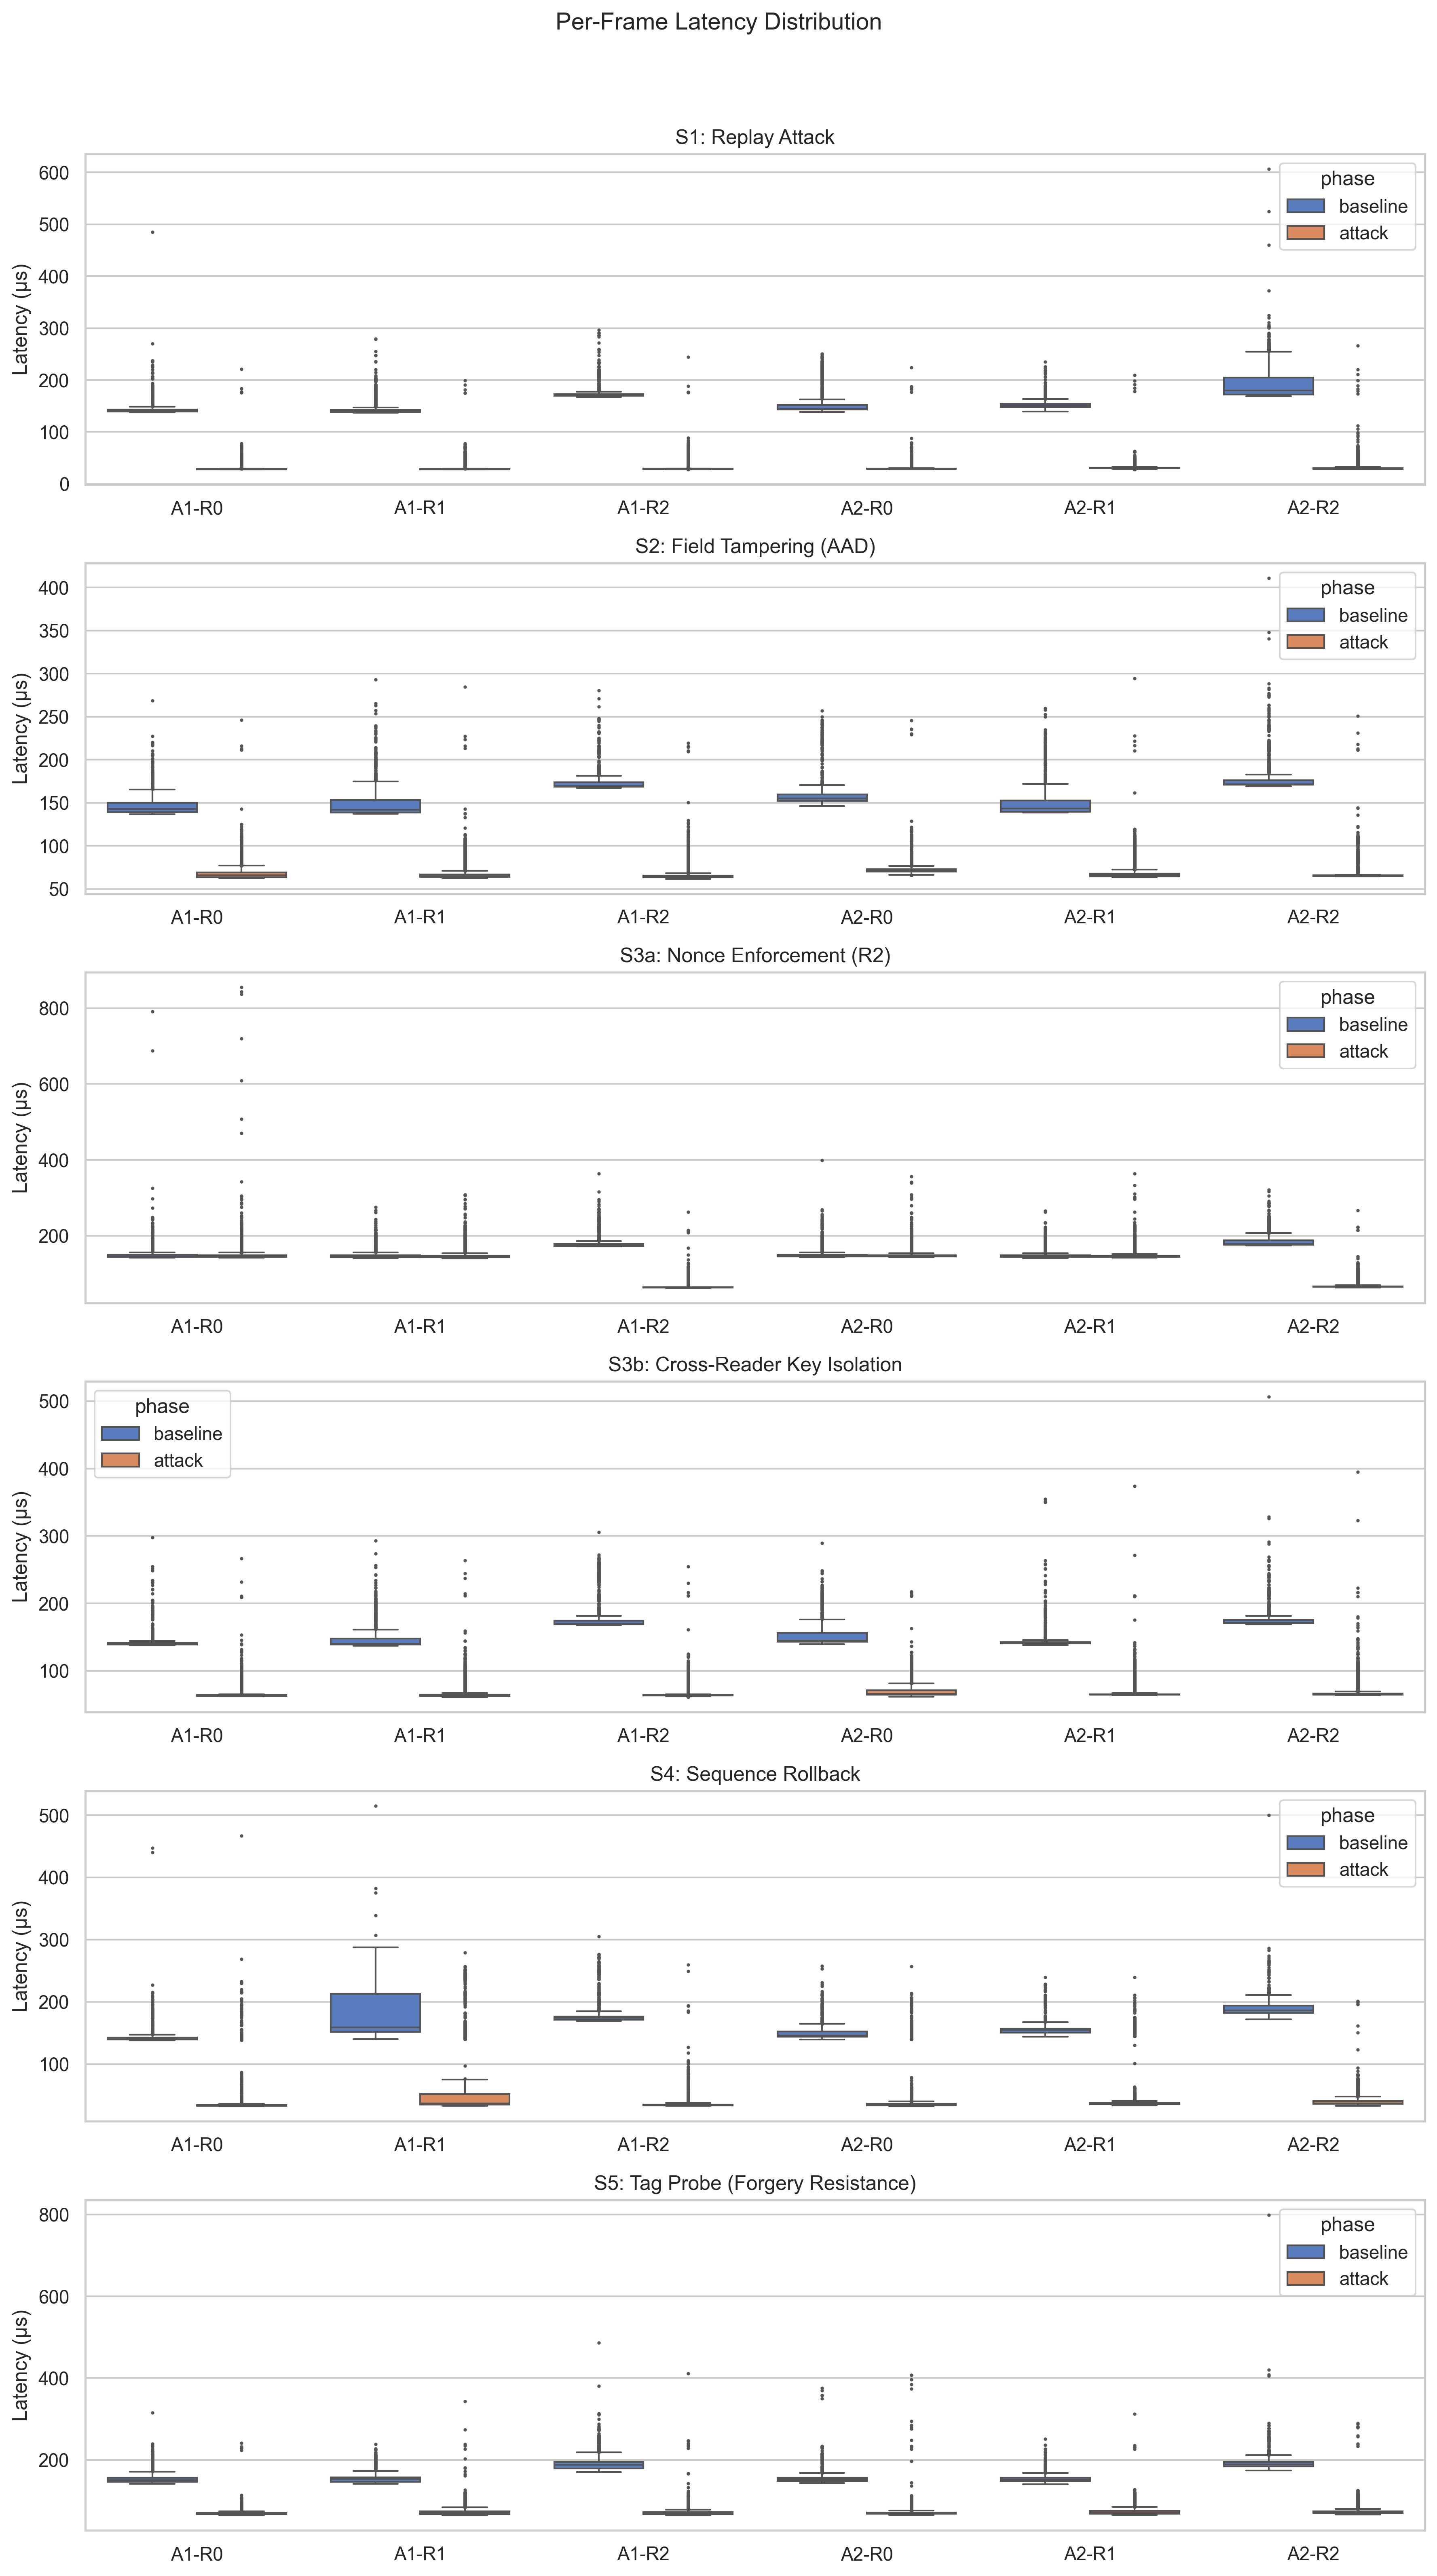
\includegraphics[width=\linewidth]{plots/latency_boxplot.png}
\caption{Distribúcia latencie podľa scenára a profilu (baseline vs.\ attack fáza, $N=500$).}
\label{fig:latency}
\end{figure}

\noindent Obrázok~\ref{fig:latency} zobrazuje boxploty latencie pre každý scenár. Viditeľný je rozdiel medzi baseline a attack fázou: pri S1 (replay) je attack latencia nižšia, pretože replay window odmietne frame skôr bez pokusu o dešifrovanie. Pri S2 a S5 je attack latencia vyššia pre R2, pretože detektor vykonáva dodatočné kontroly pred zamietnutím.

\subsection{Diskusia a interpretácia výsledkov}
\label{sec:discussion}

\subsubsection{Tézis 1: Nonce enforcement a HKDF izolácia ako dva piliere bezpečnosti}

\textbf{S3a --- nonce enforcement:} R0/R1 nemajú verifikáciu nonce; frame s chybným nonce prejde so 100\% úspešnosťou. R2 rekonštruuje očakávaný nonce a pri nesúlade okamžite zakaranténuje čítačku (0\% úspešnosť). S3a je jediný scenár, kde sa R0/R1 a~R2 správajú zásadne odlišne. V~aktuálnom jednoserverovom nasadení generátor a~verifikátor nonce zdieľajú ten istý \texttt{KeyManager} --- odchýlka nemôže nastať za normálnych okolností. Ak však systém prejde na distribuovanú architektúru (viacero serverov, oddelené generovanie a~verifikácia), vynucovaná nonce politika sa stáva kritickou poistkou proti tichému porušeniu unikátnosti nonce\cite{RogawayNonceMisuse2004}.

\textbf{S3b --- HKDF key isolation:} HKDF\cite{RFC5869} derivuje unikátny AEAD kľúč pre každú kombináciu (reader\_id, key\_version). Žiadny profil neprijal ani jeden cross-reader frame (0\% úspešnosť). R2 reaguje okamžitou karanténou (nonce kontextový nesúlad), R0/R1 odmietajú individuálne (decrypt\_failed).

\textbf{Záver:} S3a a~S3b testujú dve komplementárne osi bezpečnosti. Nonce enforcement (S3a) diferencuje nonce režimy a~zabezpečuje škálovateľnosť; HKDF izolácia (S3b) zabezpečuje compartmentalization medzi čítačkami nezávisle od nonce režimu.

\subsubsection{Tézis 2: ProtocolAnomalyDetector materiálne zvyšuje bezpečnosť}

R2 profily dosiahli 0\% úspešnosť útoku naprieč všetkými testovanými scenármi. V scenároch S3a a S4 bol R2 \textbf{jediným z testovaných mechanizmov}, ktorý útok zastavil:

\begin{itemize}[leftmargin=*,itemsep=2pt]
  \item S3a: nonce enforcement --- R0/R1 prepustia 100\%, R2 zachytí a zakaranténuje (0\%),
  \item S3b: cross-reader --- všetky profily blokujú (HKDF izolácia), R2 navyše karanténuje od prvého frame,
  \item S4: 11\% $\rightarrow$ 0\% (seq\_rollback detekcia).
\end{itemize}

\noindent V S1, S2 a S5 iné mechanizmy (replay window, AAD, AEAD tag verifikácia) tiež zamietajú škodlivé frame, ale R2 pridáva \emph{karanténu} --- čítačka je zablokovaná pre ďalšie požiadavky, nielen odmietnutý jednotlivý frame.

\textbf{Záver:} \texttt{ProtocolAnomalyDetector} nie je len doplnok k existujúcim mechanizmom. V~dvoch z~piatich testovaných útokových scenárov (S3a, S4) bol jedinou testovanou ochranou; v~S3b a~S5 pridáva operačnú eskaláciu (karanténu) k~existujúcemu kryptografickému odmietnutiu.

\subsubsection{Tézis 3: Replay window a anomálna detekcia sú komplementárne}

Scenár S4 demonštruje štruktúrnu medzeru replay window. Funkcia \texttt{ReplayWindow::contains()} kontroluje:

\begin{equation}
\text{contains}(\text{seq}) = \text{isTooOld}(\text{seq}) \lor (\text{seq} \in \text{\_seen})
\end{equation}

\noindent kde $\text{isTooOld}(\text{seq}) = (\text{seq} \leq \text{maxSeen} - W)$. Sekvenčné čísla v rollback zóne:

\begin{itemize}[leftmargin=*,itemsep=1pt]
  \item nie sú príliš staré ($> \text{maxSeen} - W$),
  \item nie sú v množine videných (nikdy neboli odoslané).
\end{itemize}

\noindent Replay window ich preto prepustí. Detektor ich zachytí cez podmienku:
\begin{equation}
\text{seq} + \delta < \text{maxSeenSeq} \implies \text{quarantine}(\texttt{seq\_rollback})
\end{equation}

\textbf{Záver:} Replay window a anomálna detekcia chránia pred rôznymi triedami útokov. Replay window odchytáva presné duplikáty. Detektor odchytáva štrukturálne anomálie (rollback, nonce mismatch, brute-force séria). Sú komplementárne, nie ekvivalentné --- v súlade s princípom vrstvených kontrol, kde každý mechanizmus pokrýva odlišnú triedu hrozieb\cite{NIST80053,DefenseInDepth}.

\subsubsection{Tézis 4: AAD binding poskytuje ochranu nezávisle od režimu nonce}

Scenár S2 ukazuje, že manipulácia \texttt{door\_id} je detekovaná \textbf{všetkými} profilmi. Mechanizmus je odlišný:
\begin{itemize}[leftmargin=*,itemsep=2pt]
  \item R0/R1: AEAD tag verification zlyhá, pretože AAD sa zmenilo $\rightarrow$ \texttt{decrypt\_failed}.
  \item R2: Deterministický nonce závisí od \texttt{door\_id} (súčasť header context). Zmena \texttt{door\_id} zmení kontext $\rightarrow$ nonce v hlavičke nezodpovedá $\rightarrow$ \texttt{nonce\_mismatch} (detekcia \emph{pred} dešifrovaním).
\end{itemize}

\textbf{Záver:} AAD binding je fundamentálna ochrana, ktorá funguje nezávisle od konfigurácie nonce a detektora. R2 ju dopĺňa skoršou detekciou.

\subsubsection{Tézis 5: Defense-in-depth cez karanténu}

Aj v scenároch, kde R0/R1 blokujú každý individuálny útočný frame (S1, S5), R2 pridáva kvalitatívne odlišnú reakciu: karanténu celej čítačky. Kým R0/R1 odmietajú frame poštučne (útočník môže pokračovať s ďalšími pokusmi), R2 po prvom detekovanom incidente zablokuje \textbf{všetku} komunikáciu z danej čítačky.

\textbf{Záver:} Karanténa mení reakciu systému z reaktívnej (odmietni frame) na proaktívnu (izoluj zariadenie). Toto je realizácia princípu defense-in-depth\cite{DefenseInDepth} --- vrstvy ochrany nepôsobia len nezávisle, ale eskalujú reakciu pri detekcii závažnejších anomálií. V prístupových systémoch, kde kompromitovaná čítačka môže generovať veľký objem požiadaviek, je izolácia zariadenia kritická\cite{NIST80094}.

\subsubsection{Tézis 6: Overhead detektora je prijateľný}

Tabuľka~\ref{tab:throughput} ukazuje overhead detektora:
\begin{itemize}[leftmargin=*,itemsep=1pt]
  \item A1: R1 (6{,}389~fps) $\rightarrow$ R2 (5{,}188~fps): $-18.8\%$
  \item A2: R1 (6{,}720~fps) $\rightarrow$ R2 (5{,}462~fps): $-18.7\%$
\end{itemize}

\noindent Aj pri najnižšej nameranej priepustnosti (A1--R2: 5{,}188~fps) systém spracuje $>$5{,}000 frame/s. Fyzický prístupový systém typicky generuje menej ako 10 udalostí za sekundu. Overhead detektora (${\sim}19\%$) je teda rádovo nepodstatný pre reálnu prevádzku, hoci nie je zanedbateľný a mal by byť zohľadnený pri nasadení s~vyššou záťažou.

\medskip
\noindent\textbf{Poznámka k porovnaniu A1 a A2.}
Namerané rozdiely v priepustnosti medzi algoritmami A1 (ChaCha20-Poly1305) a A2 (XChaCha20-Poly1305) odrážajú výkon konkrétnych implementácií v knižnici libsodium 1.0.20\cite{LibsodiumDoc}, nie inherentné vlastnosti abstraktných algoritmov. Dva faktory limitujú prenositeľnosť tohto porovnania:

\begin{enumerate}[leftmargin=*,itemsep=2pt]
  \item \textbf{Architektonický overhead XChaCha20.} XChaCha20 vykonáva pred samotným šifrovaním medzikrok HChaCha20\cite{Bernstein2012}, ktorý redukuje 192-bitový nonce na 96-bitový podkľúč. Tento krok pridáva konštantný overhead jedného volania blokovej funkcie. V inej implementácii (napríklad hardvérovom akcelerátori alebo inom softvérovom frameworku) by pomer režijných nákladov mohol byť odlišný.
  \item \textbf{Úroveň optimalizácie.} Libsodium obsahuje ručne optimalizované varianty ChaCha20 pre inštrukčné sady AVX2 a SSSE3 (adresár \texttt{dolbeau/}), ktoré sa aktivujú na platformách s podporou SIMD. Miera optimalizácie nemusí byť identická pre oba algoritmy --- napríklad HChaCha20 nemusí využívať rovnakú úroveň SIMD vektorizácie ako hlavný ChaCha20 stream. Pozorované rozdiely preto môžu čiastočne odrážať \emph{kvalitu implementácie} v libsodium, nie čistú algoritmickú zložitosť.
\end{enumerate}

\noindent Pre závery tejto práce je toto rozlíšenie nepodstatné: oba algoritmy sú ekvivalentné z hľadiska bezpečnostných metrík (scenáre S1--S5) a oba dosahujú priepustnosť rádovo prevyšujúcu požiadavky fyzického prístupového systému. Avšak pri extrapolácii nameraných výkonnostných údajov na iné platformy alebo iné kryptografické knižnice\cite{OpenSSL,BoringSSL} je potrebné vykonať nezávislé meranie.

\subsection{Porovnanie s minimalistickými implementáciami}
\label{sec:baseline_comparison}

Experimentálna matica pokrýva šesť profilov od A1-R0 po A2-R2. Pre úplnosť kontextu je užitočné zasadiť výsledky do širšieho rámca a porovnať ich s~hypotetickými minimalistickými architektúrami, ktoré sa v~praxi vyskytujú v~jednoduchých prístupových systémoch.

Uvažujeme tri referenčné úrovne ochrany:
\begin{description}[leftmargin=*,itemsep=3pt]
  \item[B0 --- bez kryptografickej ochrany:] HTTP endpoint bez podpisu požiadavky, payload prenášaný ako plaintext, žiadna anti-replay ochrana, žiadny audit.
  \item[B1 --- základný HTTPS:] HTTPS s tokenom v~hlavičke (napr.\ statický API kľúč), ale bez interného AEAD frame, bez anti-replay sekvencie a bez tamper-evident auditu. Bežný vzor pre jednoduché IoT API.
  \item[A1-R0 --- základný profil tejto práce:] Náš najjednoduchší testovaný profil. Pridáva: HMAC podpis každej požiadavky, interný AEAD frame (ChaCha20-Poly1305) s~AAD binding, sliding window anti-replay, pepper-hashed identifikátory kariet a~HMAC hash chain audit.
\end{description}

\begin{table}[htbp]
\renewcommand{\arraystretch}{1.3}
\centering
\caption{Odolnosť voči útočným scenárom podľa úrovne implementácie}
\label{tab:baseline_comparison}
\small
\begin{tabular}{l c c c c}
\toprule
\textbf{Scenár / útok} & \textbf{B0} & \textbf{B1} & \textbf{A1-R0} & \textbf{A1-R2 / A2-R2} \\
\midrule
S1 Replay           & \texttimes & \texttimes  & \checkmark & \checkmark{} + karanténa \\
S2 Tampering (AAD)  & \texttimes & čiastočne   & \checkmark & \checkmark{} (pred dekr.) \\
S3a Nonce enforcement & n/a        & n/a         & \texttimes & \checkmark \\
S3b Cross-reader     & \texttimes & \texttimes  & \checkmark & \checkmark{} + karanténa \\
S4 Seq rollback     & \texttimes & \texttimes  & čiastočne  & \checkmark \\
S5 Tag probe        & \texttimes & \texttimes  & \checkmark & \checkmark{} + karanténa \\
Manipulácia auditu  & \texttimes & \texttimes  & \checkmark & \checkmark \\
Identita karty (DB) & \texttimes & \texttimes  & \checkmark{} (HMAC) & \checkmark \\
\bottomrule
\end{tabular}
\end{table}

Z~tabuľky vyplývajú tri závery. Po prvé, prechod z~B0 na A1-R0 predstavuje kvalitatívny skok: väčšina útočných scenárov (S1, S2, S3, S5, audit, identita) je zastavená bez nutnosti nasadiť R2. Po druhé, plná ochrana pri S4 vyžaduje R2 detektor --- jednoduché AEAD bez anomálnej detekcie nestačí na detekciu seq rollback. Po tretie, karanténa v~R2 profiloch mení charakter odpovede systému z~per-frame odmietania na izoláciu celého zariadenia, čo je realizáciou princípu \emph{defense-in-depth}\cite{DefenseInDepth,NIST80053}.

B1 (HTTPS bez interného AEAD) chráni pred pasívnym odpočúvačom na sieťovej vrstve, no nevyrieši scenáre, kde je komunikácia legitimná na transportnej vrstve ale manipulovaná na aplikačnej --- presne to, čo demonštrujú S1--S5. Interný AEAD frame a~anti-replay sú teda komplementárne k~TLS, nie jeho náhradou\cite{RFC9325}.

\subsection{Zhrnutie experimentov}

\begin{figure}[htbp]
\centering
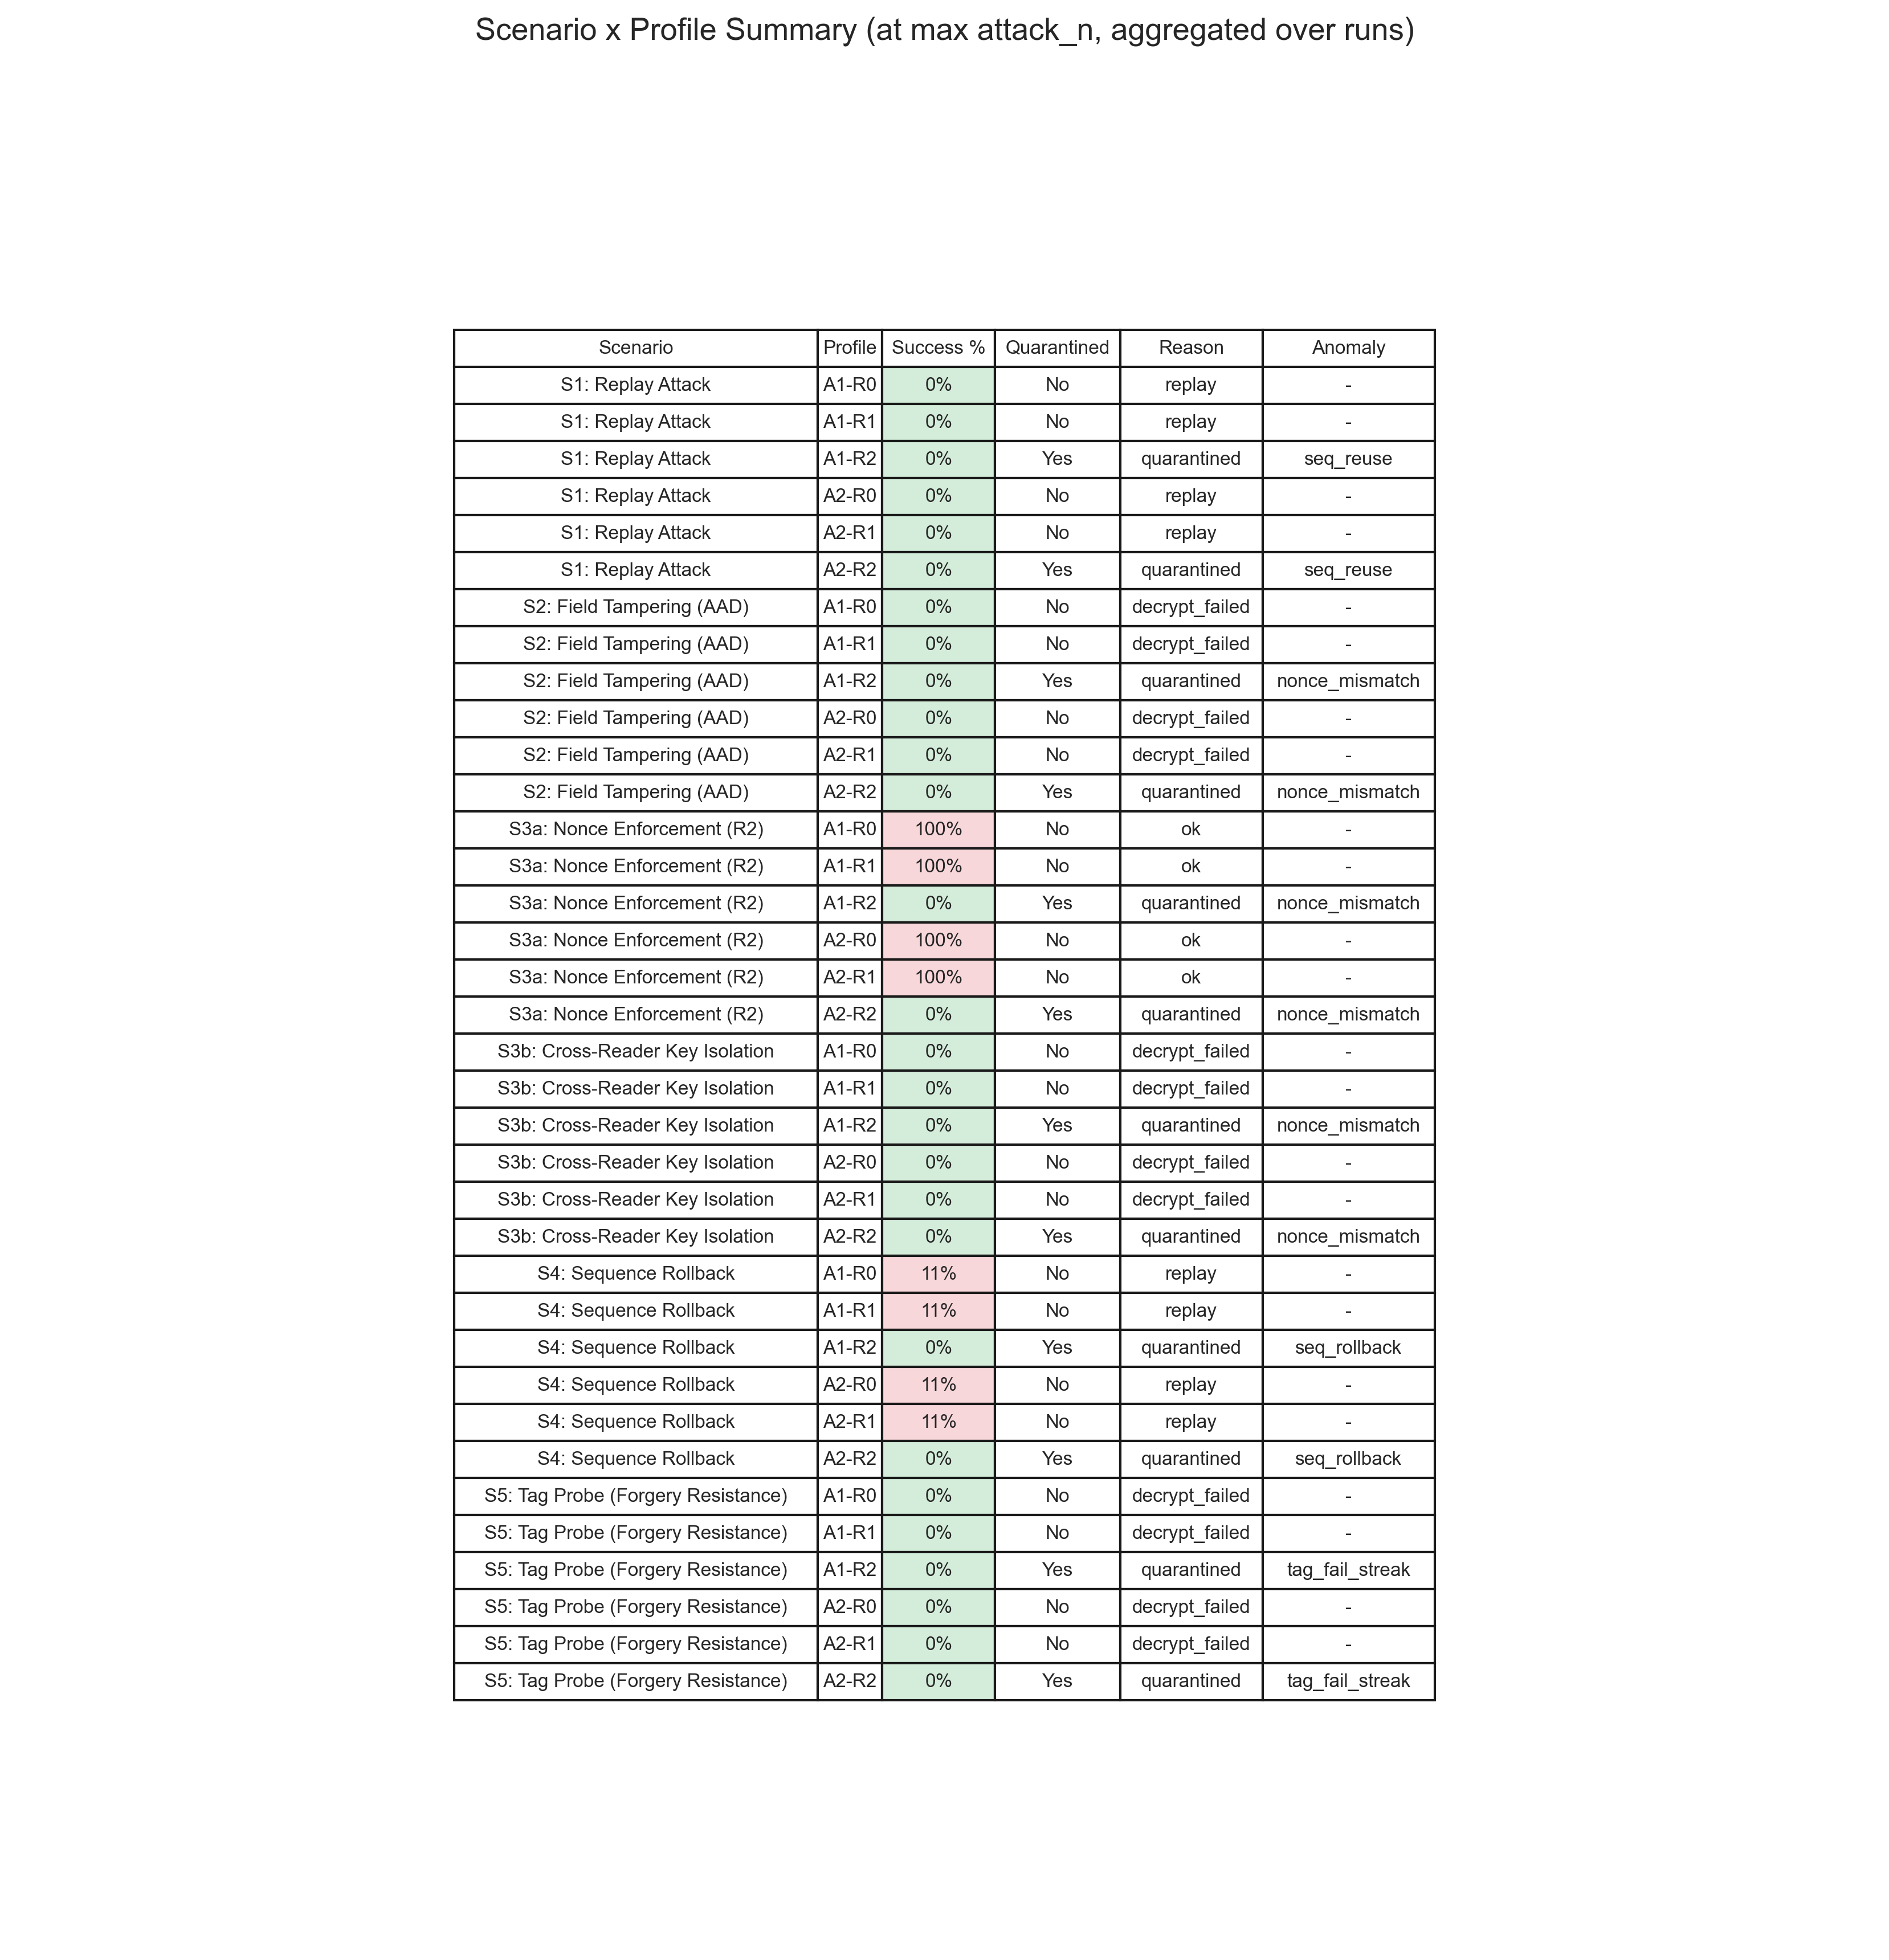
\includegraphics[width=\linewidth]{plots/scenario_summary_table.png}
\caption{Súhrnná tabuľka výsledkov experimentov: scenár $\times$ profil.}
\label{fig:summary_table}
\end{figure}

\noindent Obrázok~\ref{fig:summary_table} poskytuje prehľad výsledkov všetkých scenárov a profilov. Experimentálna analýza šiestich scenárov naprieč šiestimi konfiguračnými profilmi potvrdila nasledujúce zistenia:

\begin{enumerate}[leftmargin=*,itemsep=2pt]
  \item \textbf{Nulová false reject rate:} Žiadny validný frame nebol zamietnutý žiadnym profilom.
  \item \textbf{Nonce enforcement a HKDF izolácia (S3a/S3b):} S3a ukazuje, že R2 ako jediný vynucuje nonce politiku --- poistka pre budúce škálovanie. S3b potvrdzuje, že HKDF per-reader derivácia izoluje kľúčový materiál medzi čítačkami naprieč všetkými profilmi.
  \item \textbf{R2 zablokoval všetky testované scenáre:} 0\% úspešnosť naprieč S1--S5 v~rámci tejto experimentálnej sady (vrátane S3a, ktorý je komponentovou validáciou nonce mechanizmu, nie simuláciou externého útoku).
  \item \textbf{Replay window a detektor sú komplementárne:} S4 odhaľuje štruktúrnu medzeru replay window, ktorú detektor uzatvára.
  \item \textbf{AAD binding je fundamentálna ochrana:} Funguje nezávisle od nonce režimu.
  \item \textbf{Karanténa pridáva proaktívnu izoláciu zariadení:} Kvalitativne odlišná od per-frame odmietnutia.
  \item \textbf{Overhead detektora (${\sim}19\%$):} Pri reálnej záťaži prístupového systému ($<$10 udalostí/s) rádovo nepodstatný; pri vyššej záťaži by mal byť zohľadnený.
  \item \textbf{Výsledky sú reprodukovateľné:} Všetkých 5 behov (seedy 42--46) poskytlo zhodné výsledky attack success rate. Bezpečnostné mechanizmy sú invariantné voči hodnotám nonce --- 5 behov tu neplní úlohu štatistického vzorku, ale overenia konzistencie výsledkov.
\end{enumerate}

Tieto výsledky potvrdujú pôvodnú hypotézu práce: kombinácia AEAD s AAD binding, deterministickým nonce a runtime anomálnou detekciou (profil R2) \textbf{materiálne zvyšuje odolnosť} prístupového systému v porovnaní so základnými konfiguráciami, a to pri prijateľnom výkonnostnom overheade.
